%====================================================================%
%                  MORIOND.TEX                                       %
%====================================================================%

\documentclass{moriond}

\usepackage{subcaption}
\captionsetup{compatibility=false}

\bibliographystyle{unsrt}    
% for BibTeX - sorted numerical labels by order of
% first citation.

% A useful Journal macro
\def\Journal#1#2#3#4{{#1} {\bf #2}, #3 (#4)}

% Some useful journal names
\def\NCA{\em Nuovo Cimento}
\def\NIM{\em Nucl. Instrum. Methods}
\def\NIMA{{\em Nucl. Instrum. Methods} A}
\def\NPB{{\em Nucl. Phys.} B}
\def\PLB{{\em Phys. Lett.}  B}
\def\PRL{\em Phys. Rev. Lett.}
\def\PRD{{\em Phys. Rev.} D}
\def\ZPC{{\em Z. Phys.} C}

% Some other macros used in the sample text
\def\st{\scriptstyle}
\def\sst{\scriptscriptstyle}
\def\mco{\multicolumn}
\def\epp{\epsilon^{\prime}}
\def\vep{\varepsilon}
\def\ra{\rightarrow}
\def\ppg{\pi^+\pi^-\gamma}
\def\vp{{\bf p}}
\def\ko{K^0}
\def\kb{\bar{K^0}}
\def\al{\alpha}
\def\ab{\bar{\alpha}}
\def\be{\begin{equation}}
\def\ee{\end{equation}}
\def\bea{\begin{eqnarray}}
\def\eea{\end{eqnarray}}
\def\CPbar{\hbox{{\rm CP}\hskip-1.80em{/}}}
%temp replacement due to no font
%%%%%%%%%%%%%%%%%%%%%%%%%%%%%%%%%%%%%%%%%%%%%%%%%%
%                                                %
%    BEGINNING OF TEXT                           %
%                                                %
%%%%%%%%%%%%%%%%%%%%%%%%%%%%%%%%%%%%%%%%%%%%%%%%%%

%\newcommand{\Photo}{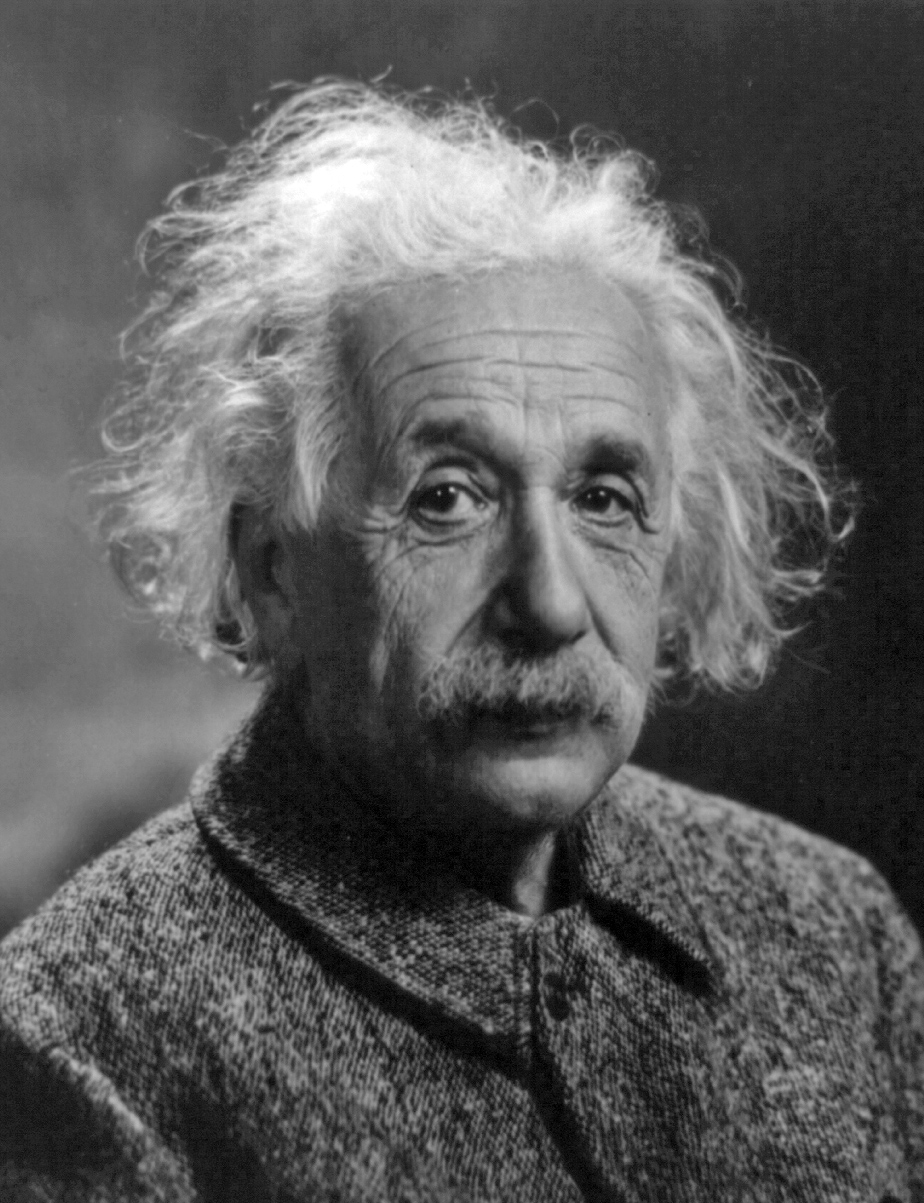
\includegraphics[height=35mm]{mypicture}}
\newcommand{\Photo}{}

\begin{document}
\title{Highlights of ATLAS Search Results}

\author{Bingxuan Liu, on behalf of the ATLAS Collaboration}

\address{Department of Physics, Simon Fraser University, Vancouver, Canada}

\maketitle\abstracts{Searching for beyond standard model (BSM) physics has been
one of the primary goals of the Large Hadron Collider (LHC) physics program.
The LHC delivered 140 $\mathrm{fb}^{-1}$ data of high quality in Run 2,
allowing both the ATLAS and CMS collaborations to expand and improve their
search programs. The recent development in detector perforamnce and analysis
techniques have brought significant boosts to the search sensitivities. In this
article, highlights of recent ATLAS search results are discussed and
summarized.}  

\section{Introduction}

Many mysteries in particle physics, such as the hierarchy problem, the origin
of dark matter (DM) and neutrino masses are still waiting for answers or hints
from the Large Hadron Collider (LHC). ATLAS is a general purpose detector at
the LHC that is capable of searching for beyond standard model (BSM) physics
via various approaches. ATLAS has conducted a comprehensive set of searches in
the past years, excluding the majority part of the phase space. As a
consequence, recent ATLAS searches are featured with applying cutting-edge
analysis techniques or detector performance development, filling the gaps
between explored regions of phase space and considering challenging, completely
uncovered signatures.      

\section{Full Run 2 Upgrades}

The detector performance in ATLAS is continuously improving, thanks to the
diligent work carried out in the relevant areas. For instance, the performance
of bottom- and top-tagging has advance significantly in the past few years. In
addition, the application of machine learning techniques have become very
mature in physics analyses, enhancing the sensitivities. Even though previous
analyses have explored similar final states, taking advantage of the above
facts and more data, the full Run 2 upgrades of the those searches will push
the exclusion limits further.\\

In the full Run 2 ATLAS vector-like quark search, the top partner masses with
50\% decay width are excluded up to 1975 GeV for the singlet representation,
considering $B(T\rightarrow Wb)=0.5$, as shown in
Figure (~\ref{fig:limits1}~\subref{fig:vlq}). Compared to the previous analysis
probing the same final state, this analysis adopted an updated top-tagger and
more optimized selections, achieving greatly improved exclusion limits. The
ATLAS full Run 2 right-handed neutrino search sets the most stringent limits on
the Keung-Senjanović process in the TeV $W$ partner ($W_{\mathrm{R}}$) mass
region. This search considers both the ``resolved'' and ``merged'' cases,
depending on the mass split between the $W_{\mathrm{R}}$ and the heavy neutrino
($N_{\mathrm{R}}$). For Majorana neutrinos, in the muon channel, the limit on
$m(W_{\mathrm{R}})$ reaches 6.4 TeV for $m(N_{\mathrm{R}})=1$ TeV, and the
limit on $m(N_{\mathrm{R}})$ extends to 3.6 teV for $m(W_{\mathrm{R}})=4.8$
TeV, as shown in Figure (~\ref{fig:limits1}~\subref{fig:rhn}).\\           

Combination of different analyses offers a powerful way to constrain a given
type of model. A recent ATLAS search considers final states with $\tau$ leptons
and hadronic jets, providing interpretation including both the leptoquark and
excited $\tau$ models. In particular, it is sensitive to $LQ\rightarrow
c\tau^{-}$ ($\overline{LQ}\rightarrow\overline{c}\tau^{+}$) decays, as the
analysis does not enforce any jets to be $b$-tagged. It comprises a critical
piece in the leptoquark combination given this unique feature of the signal
region selection. As seen in Figure (~\ref{fig:limits1}~\subref{fig:micro}),
$LQ$ masses below 1.3 TeV are excluded, assuming the branching ratio of their
decays to the $c$-quark–$\tau$-lepton pair is equal to one.\\   

\clearpage

\begin{figure}[htp]
     \centering
     \begin{subfigure}[b]{0.32\textwidth}
         \centering
         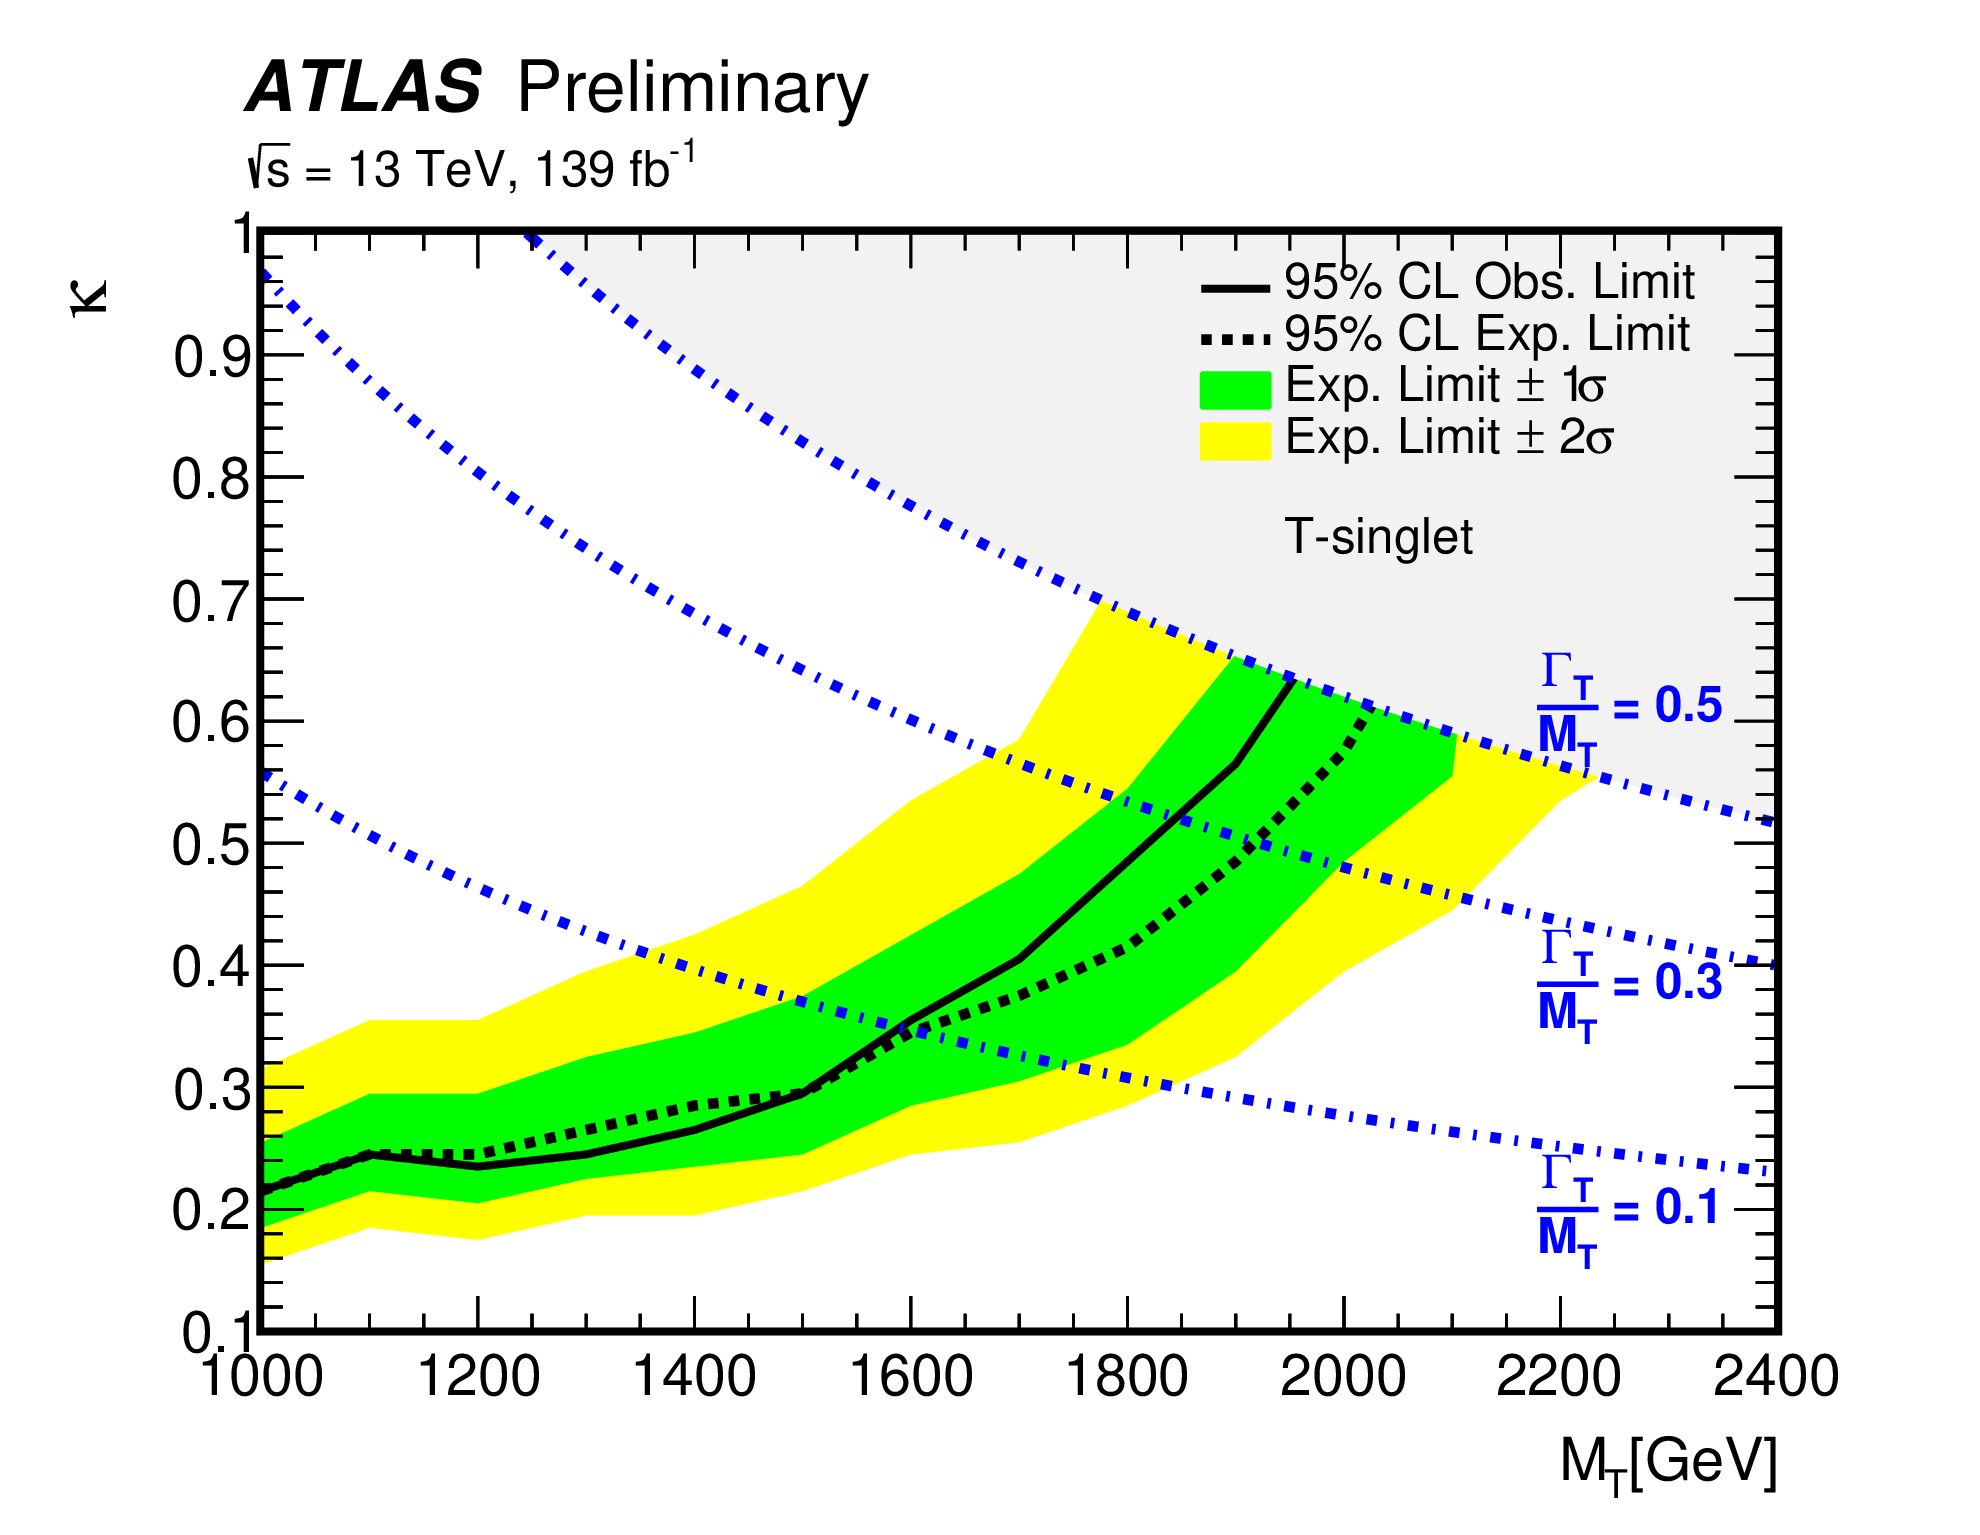
\includegraphics[width=\textwidth]{VLQ}
         \caption{}
         \label{fig:vlq}
     \end{subfigure}
     \begin{subfigure}[b]{0.32\textwidth}
         \centering
         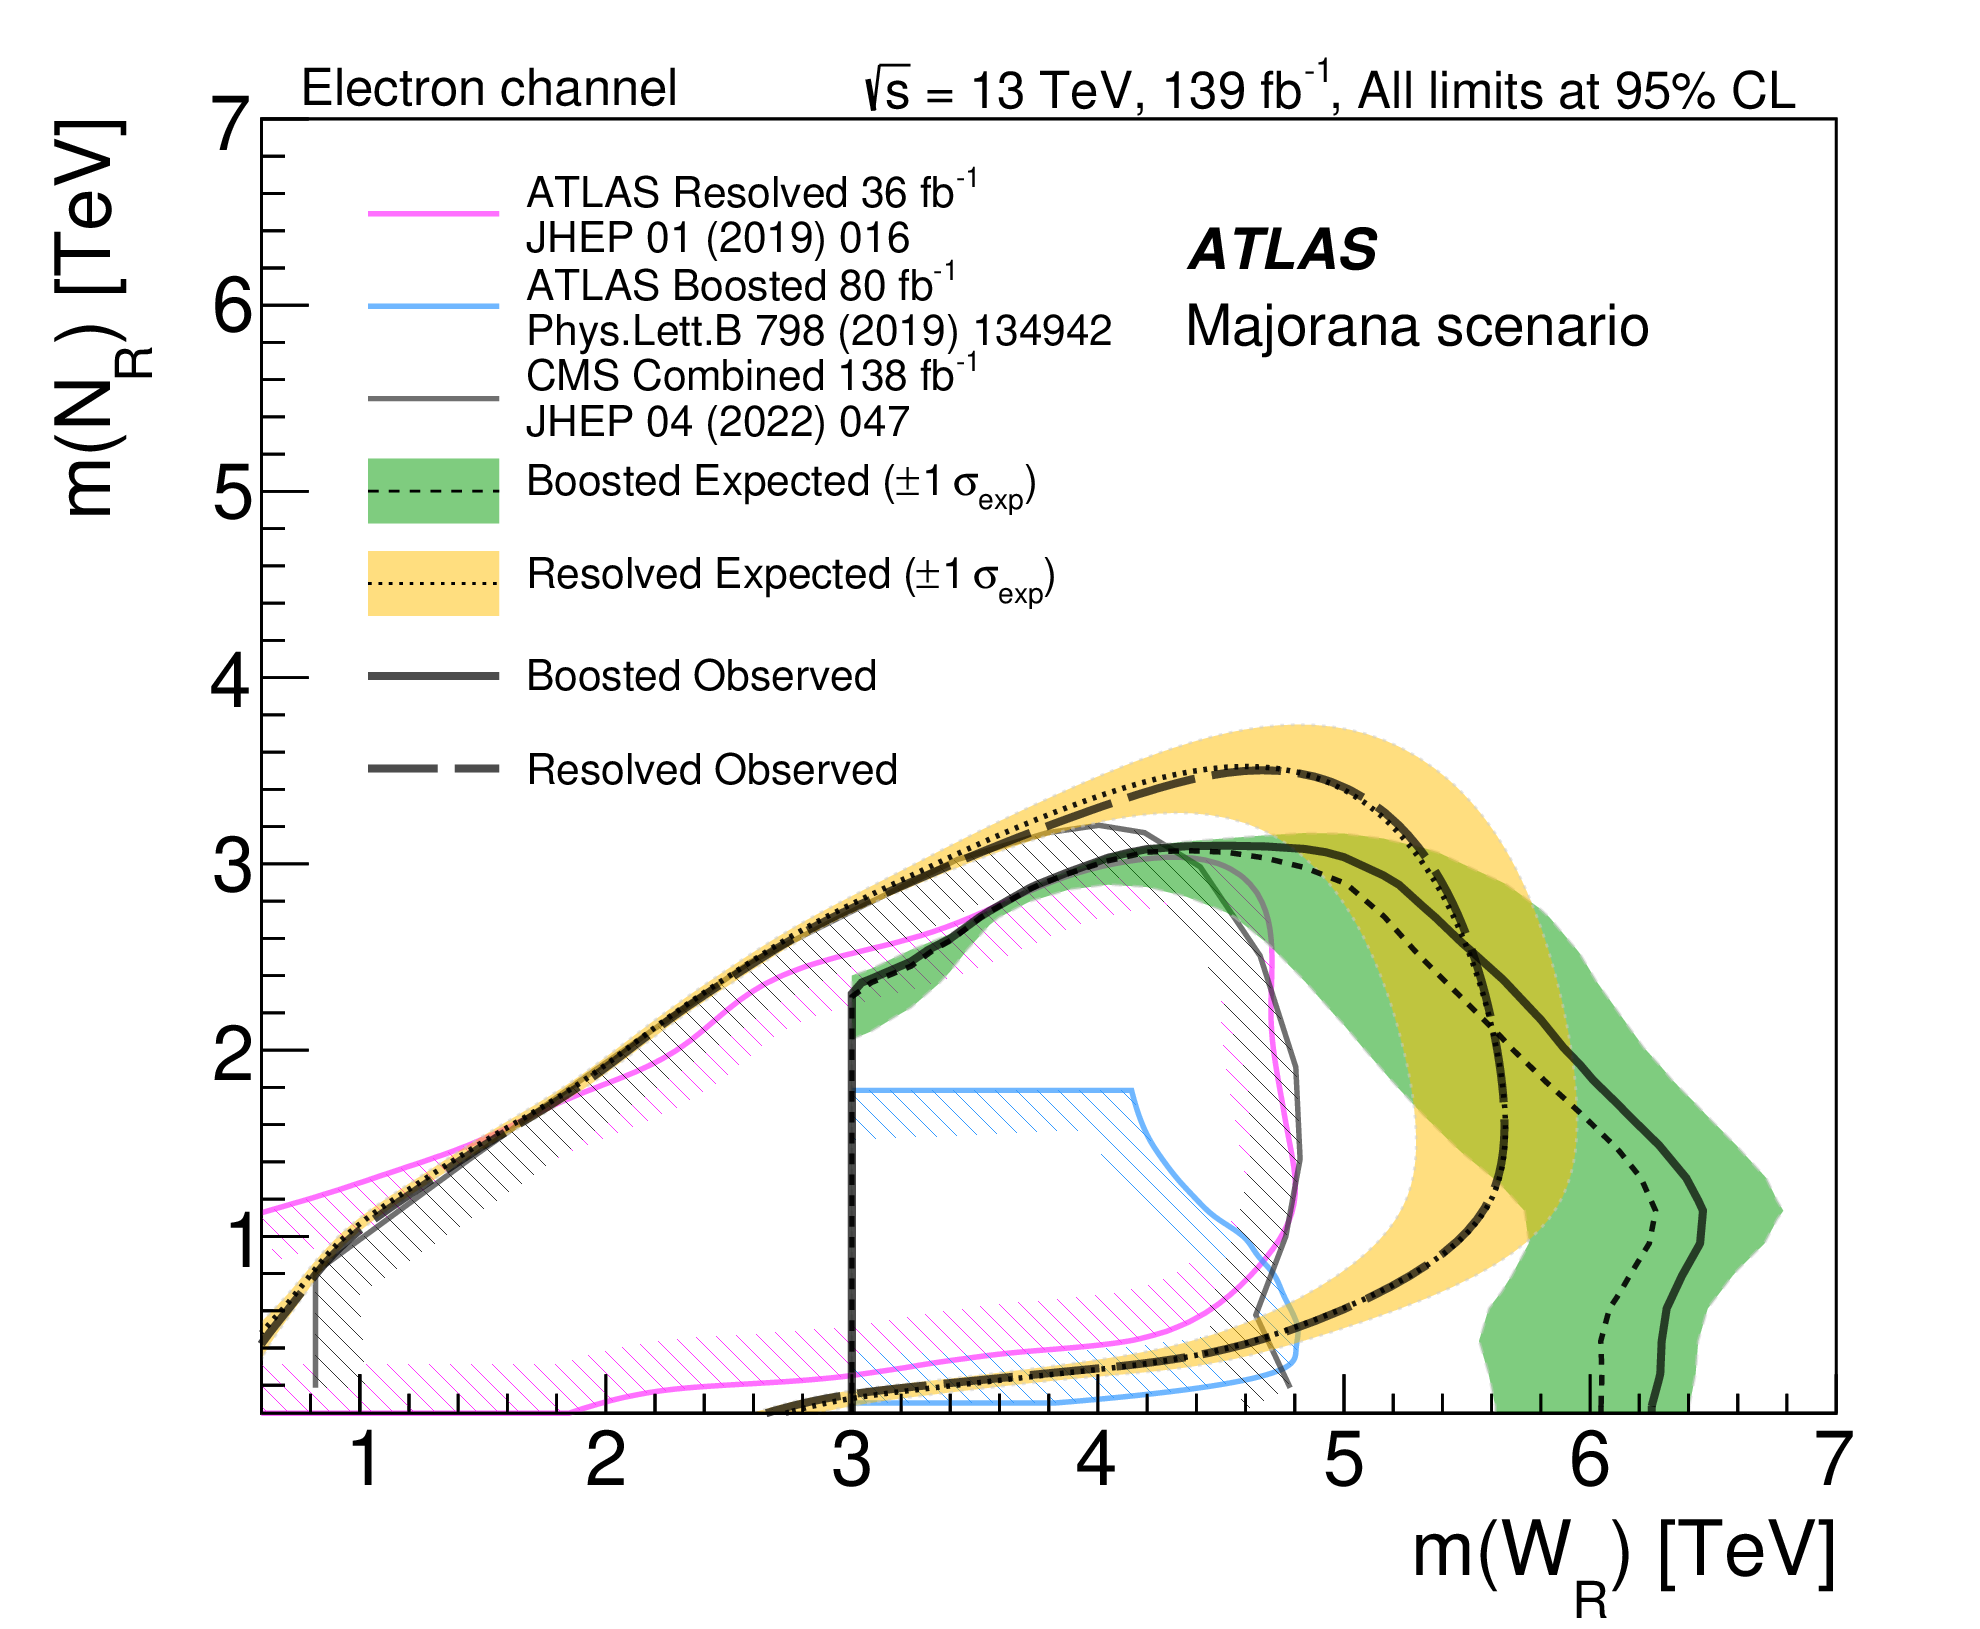
\includegraphics[width=\textwidth]{RHN}
         \caption{}
         \label{fig:rhn}
     \end{subfigure}
     \begin{subfigure}[b]{0.32\textwidth}
         \centering
         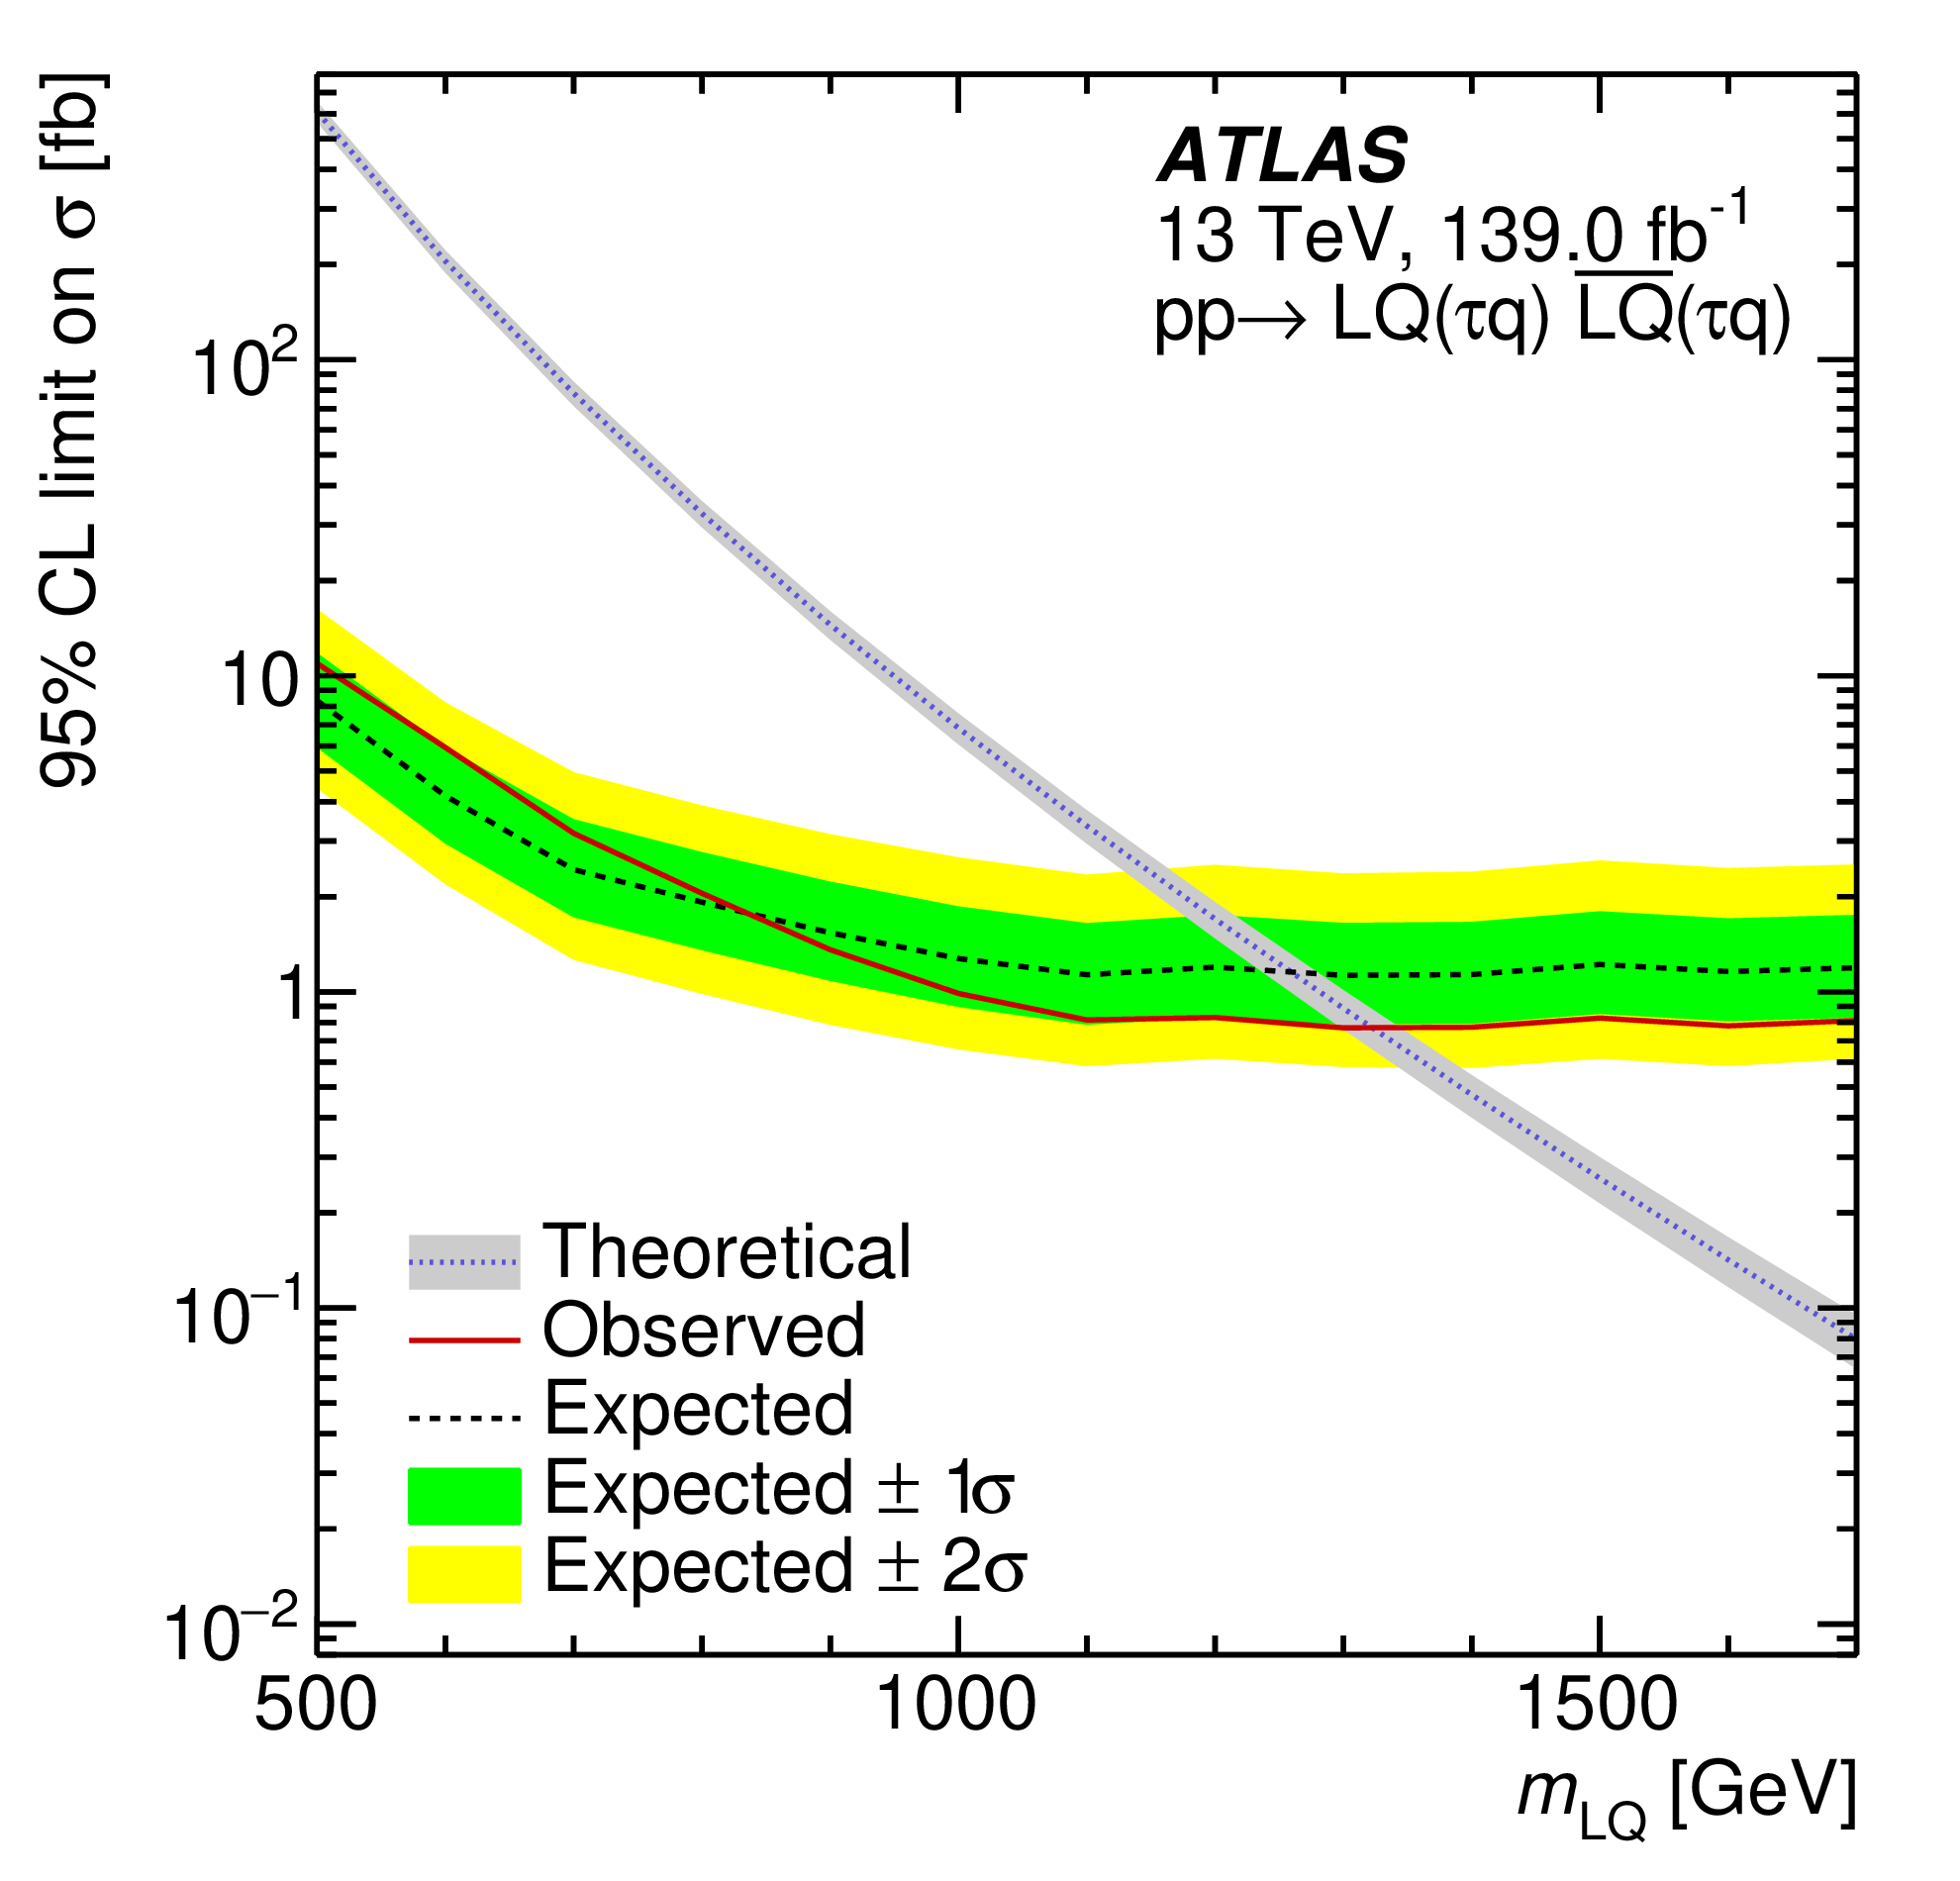
\includegraphics[width=\textwidth]{excited}
         \caption{}
         \label{fig:excited}
     \end{subfigure}
        \caption{}
        \label{fig:limits1}
\end{figure}
\section{Filling the Gap}

There have been many BSM models proposed by the theory community in the past
decades. The number of free parameters in those models is so vastly large that
a single search can only probe a subset of the parameter space, a particular
combination of masses and couplings. Naturally, there are gap between exisitng
searches, and they need to be explored. The gap regions are usually hard to
probe so that special analysis strategies are essential.\\

Supersymmetry has been explored extensively at the LHC by a comprehensive
program. However various uncovered corners have been present on specific
parameter planes. A recent ATLAS search for higgsino considers the
$b\overline{b}\gamma\gamma$ final state, taking advantage of the excellent mass
resolution of the photons and the large $H\rightarrow b\overline{b}$ branching
ratio. It successfully filled the gap in the low mass region, as seen in Figure
(~\ref{fig:limits2}~\subref{fig:bbyy}).\\

The gap between dedicated long-lived particle (LLP) searches and conventional
searches is becoming increasingly important. A recent ATLAS search for
micro-displaced muons probed this region using muons reconstructed by the
standard algorithms, requiring the impact parameter ($|d_{0}|$) of the muons to
be between 0.1 and 3 mm. Control regions, validation regions, and signal
regions are constructed using the muon $|d_{0}|$ and muon-pair mass. In the
context of a smuon pair production, the smuon lifetimes down to 1 $ps$ and
smuon masses up to 520 GeV are excluded, as shown in Figure
(~\ref{fig:limits2}~\subref{fig:micro}).\\   

\begin{figure}[htp]
     \centering
     \begin{subfigure}[b]{0.32\textwidth}
         \centering
         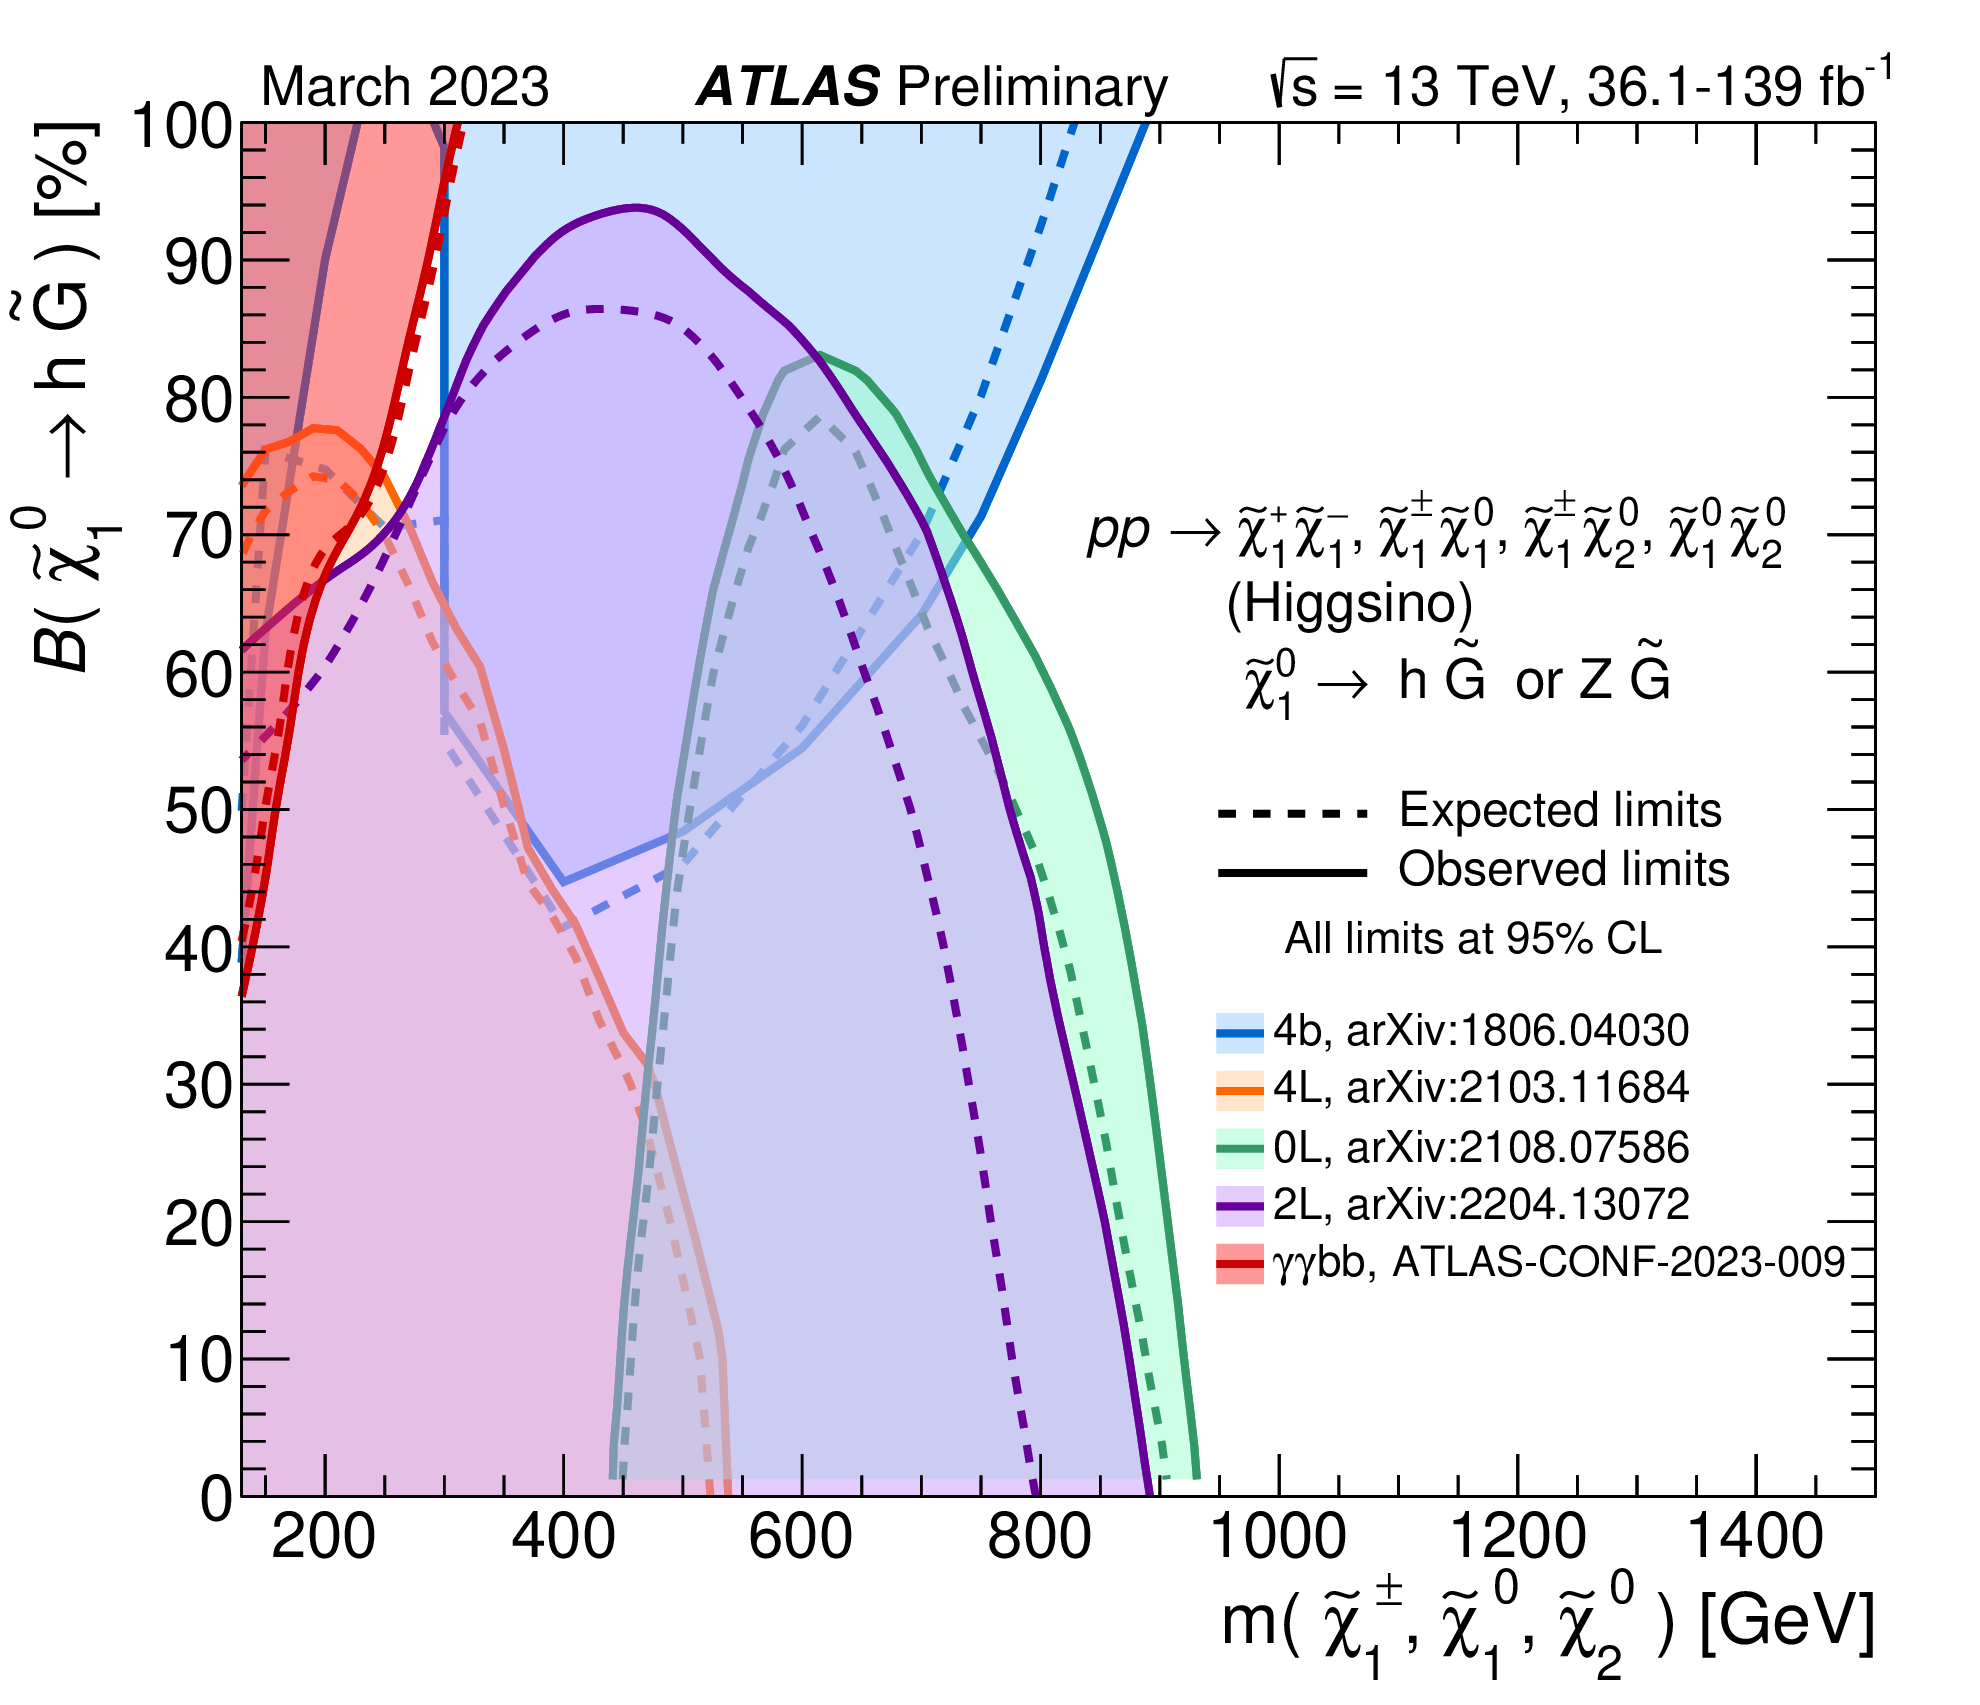
\includegraphics[width=\textwidth]{bbyy}
         \caption{}
         \label{fig:bbyy}
     \end{subfigure}
     \begin{subfigure}[b]{0.32\textwidth}
         \centering
         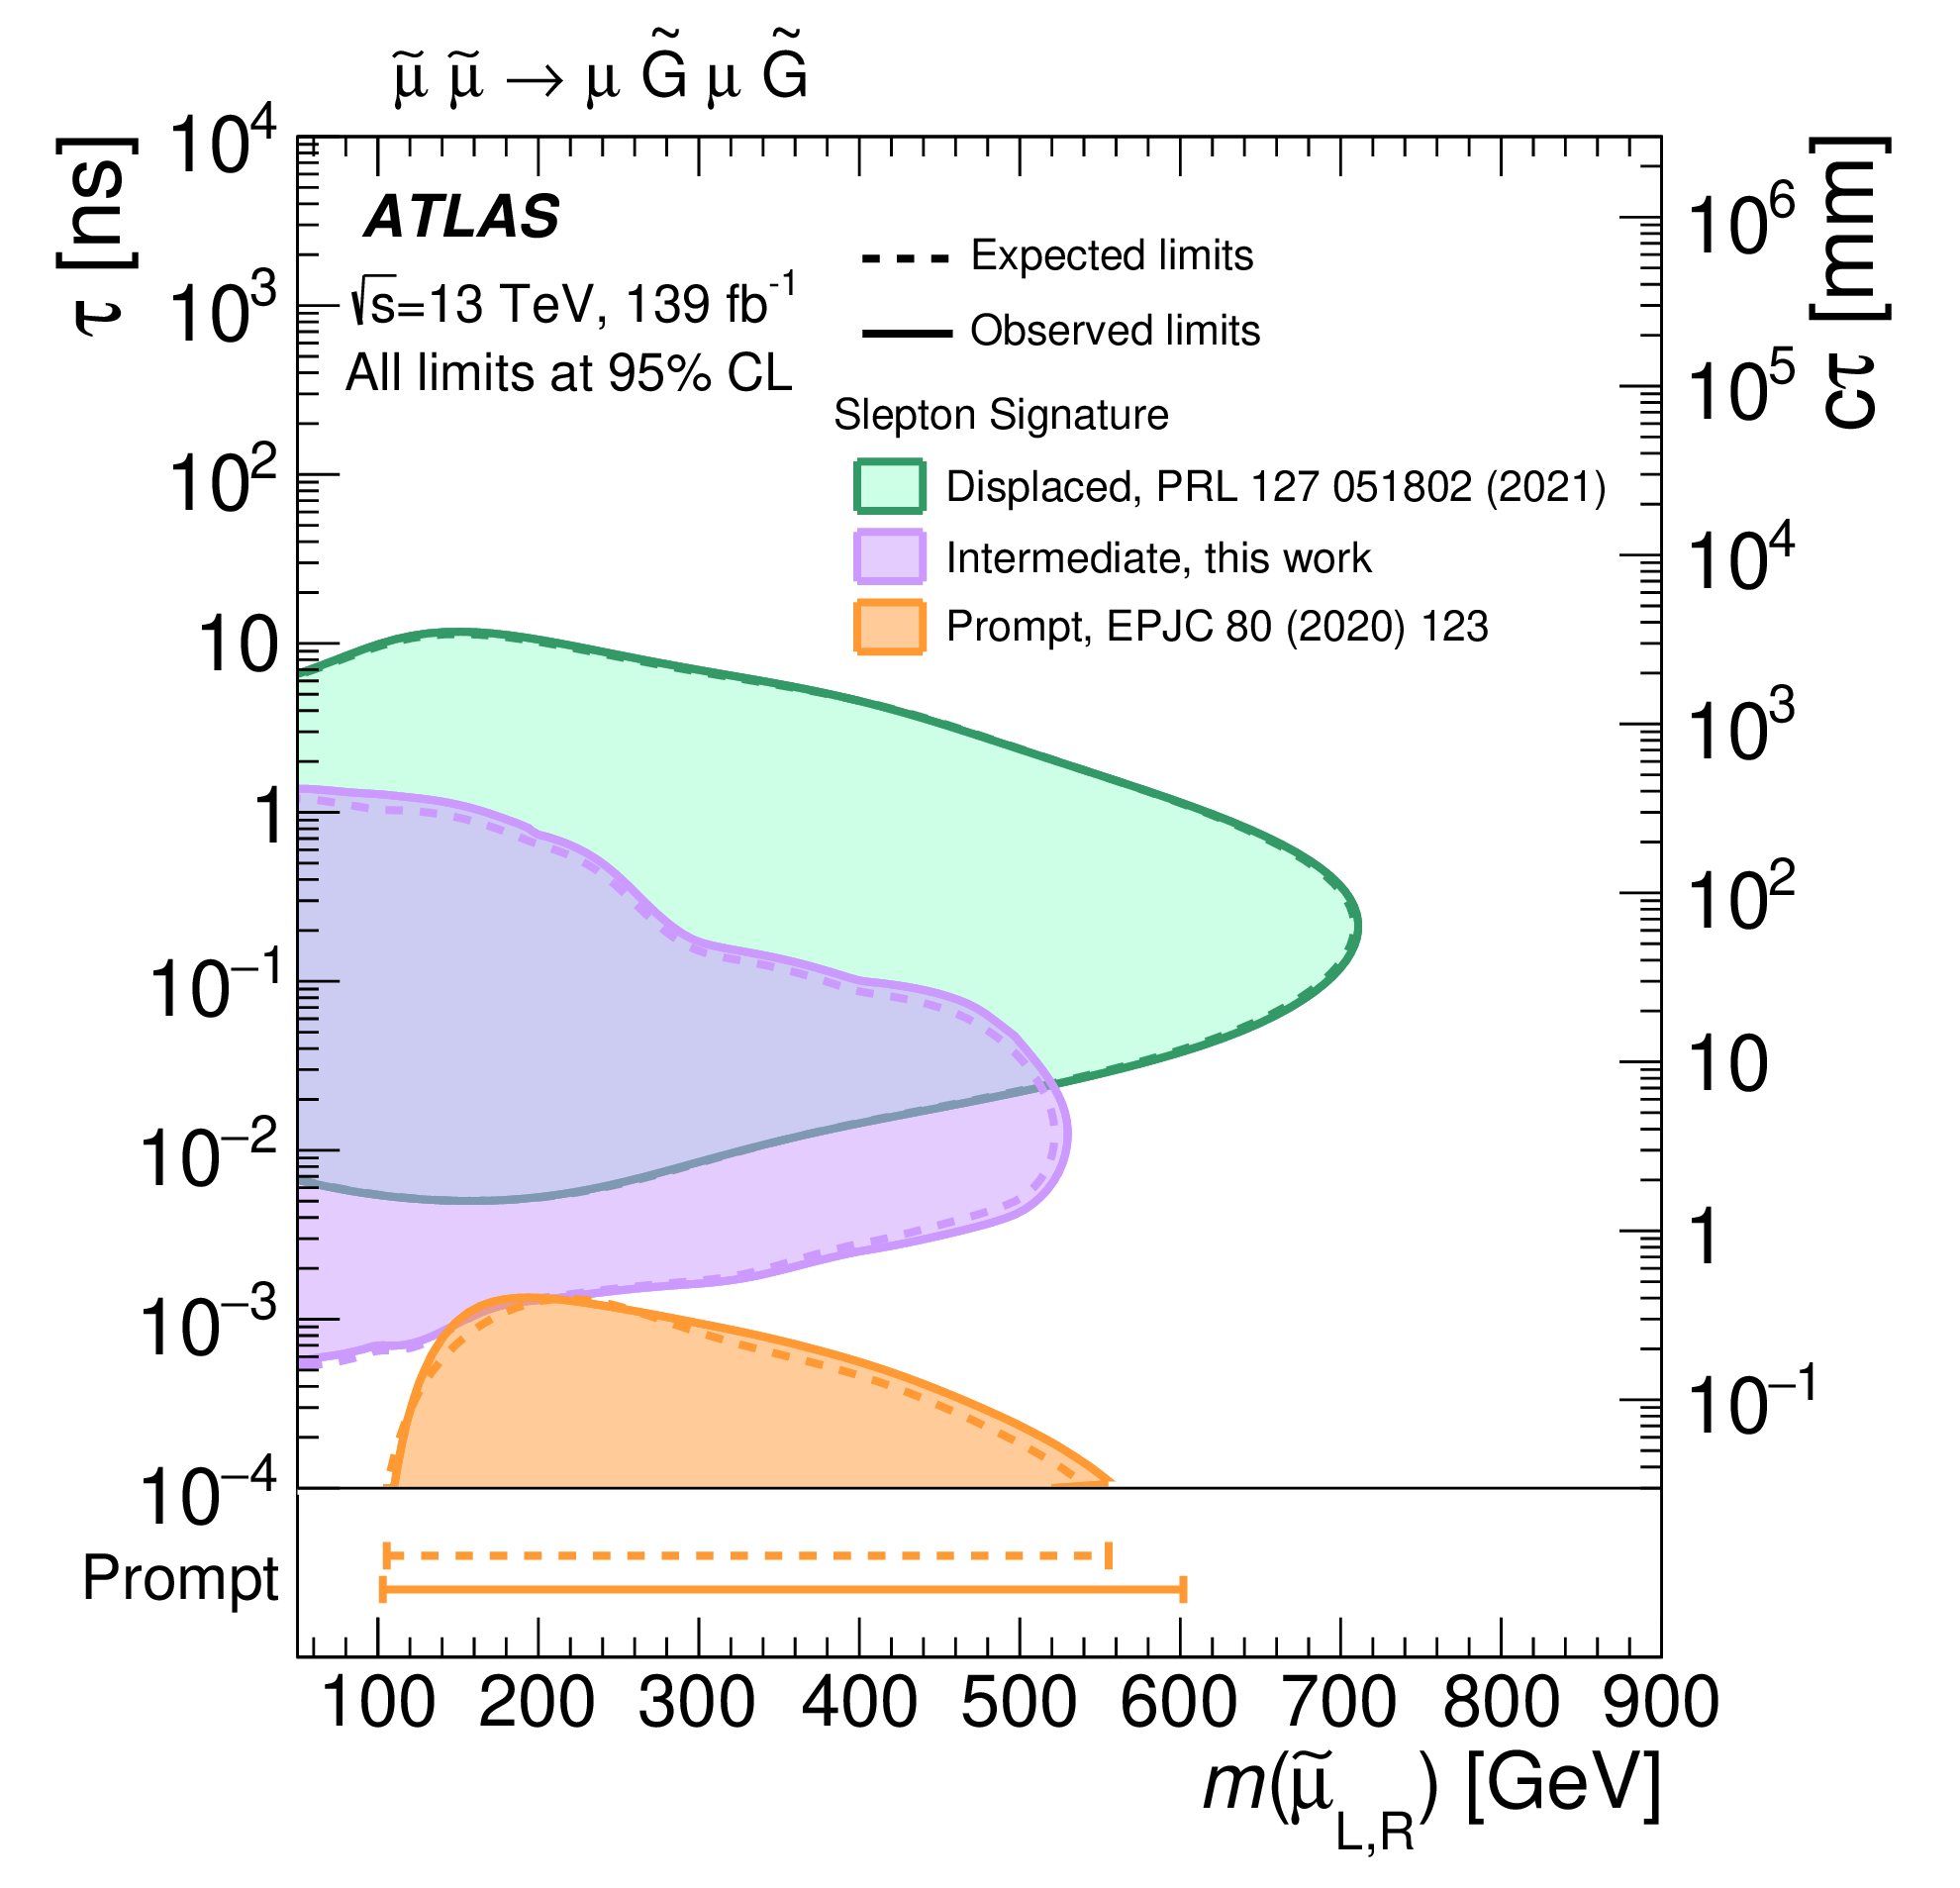
\includegraphics[width=\textwidth]{micro}
         \caption{}
         \label{fig:micro}
     \end{subfigure}
     \begin{subfigure}[b]{0.32\textwidth}
         \centering
         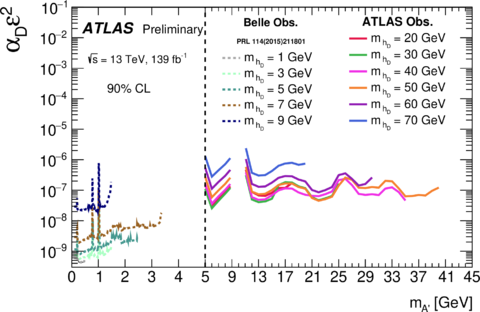
\includegraphics[width=\textwidth]{dark}
         \caption{}
         \label{fig:micro}
     \end{subfigure}
        \caption{Three simple graphs}
        \label{fig:limits2}
\end{figure}

\section{New and Challenging Signatures}

\begin{figure}[htp]
     \centering
     \begin{subfigure}[b]{0.32\textwidth}
         \centering
         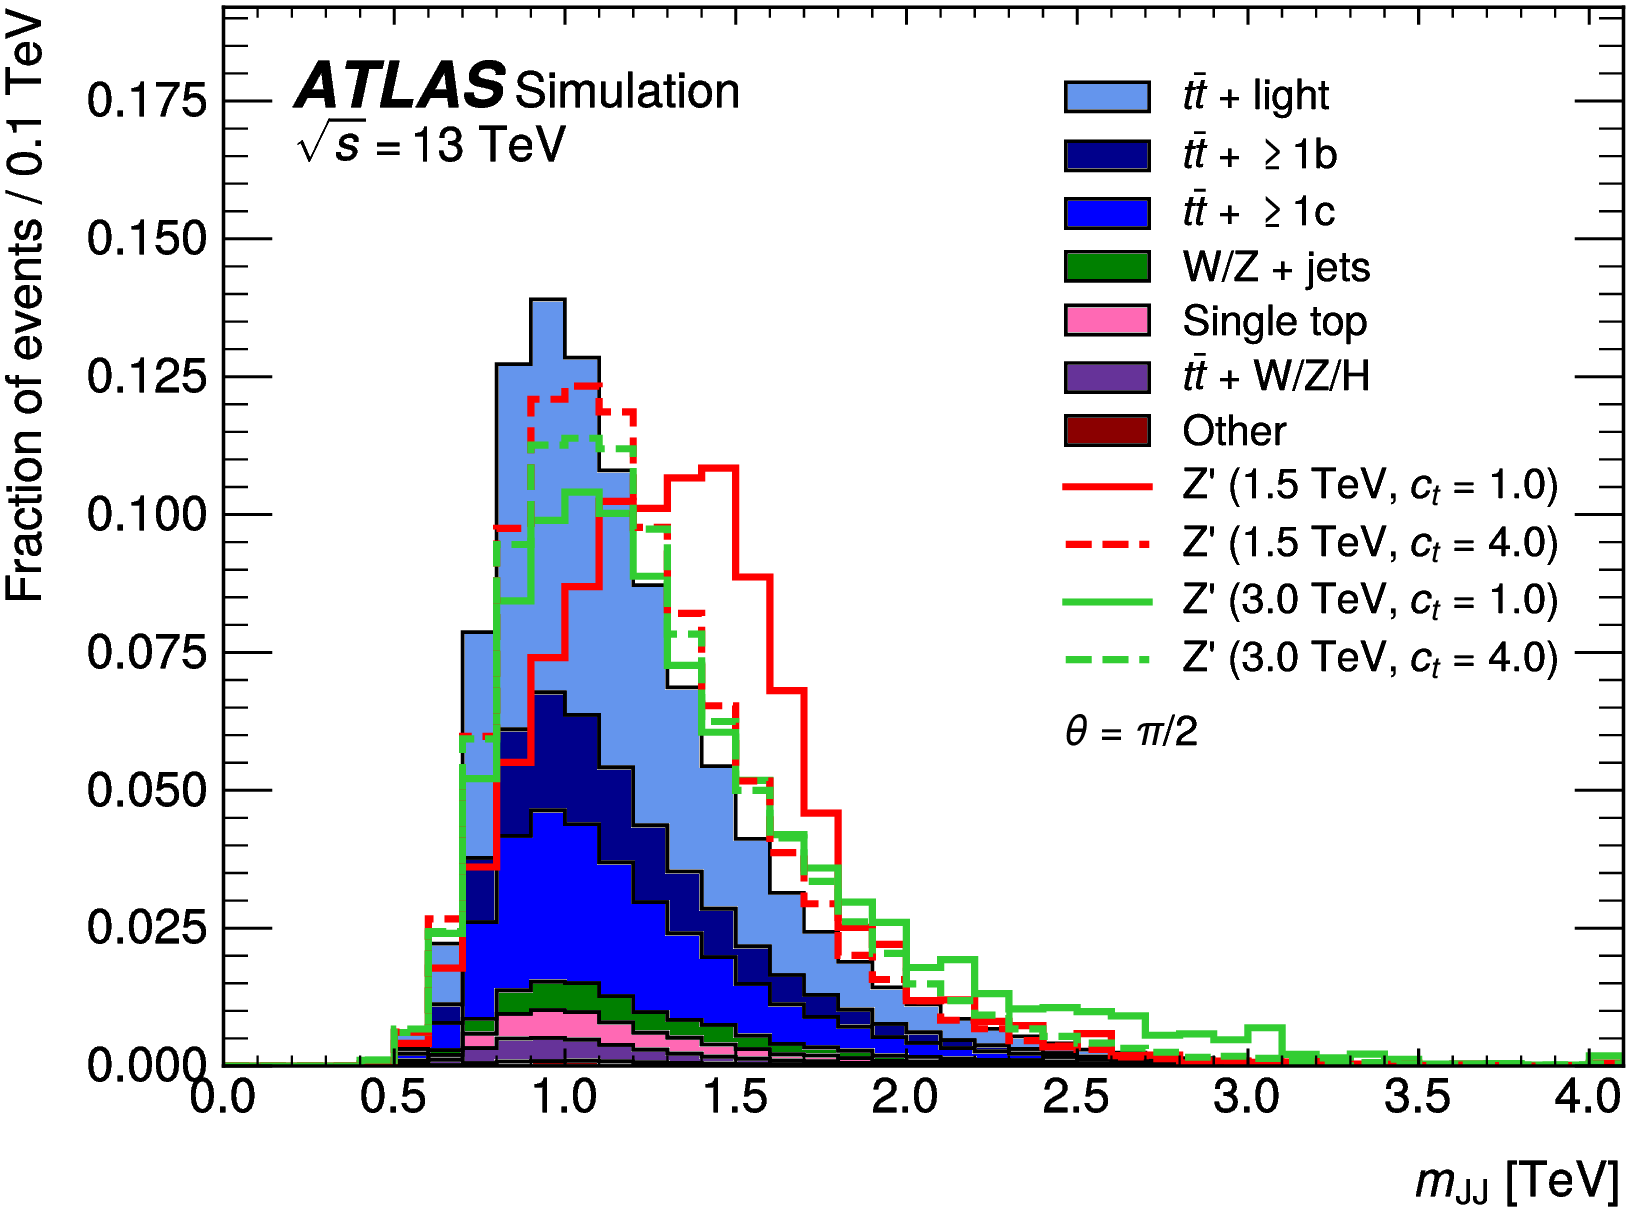
\includegraphics[width=\textwidth]{mass}
         \caption{}
         \label{fig:mass}
     \end{subfigure}
     \begin{subfigure}[b]{0.32\textwidth}
         \centering
         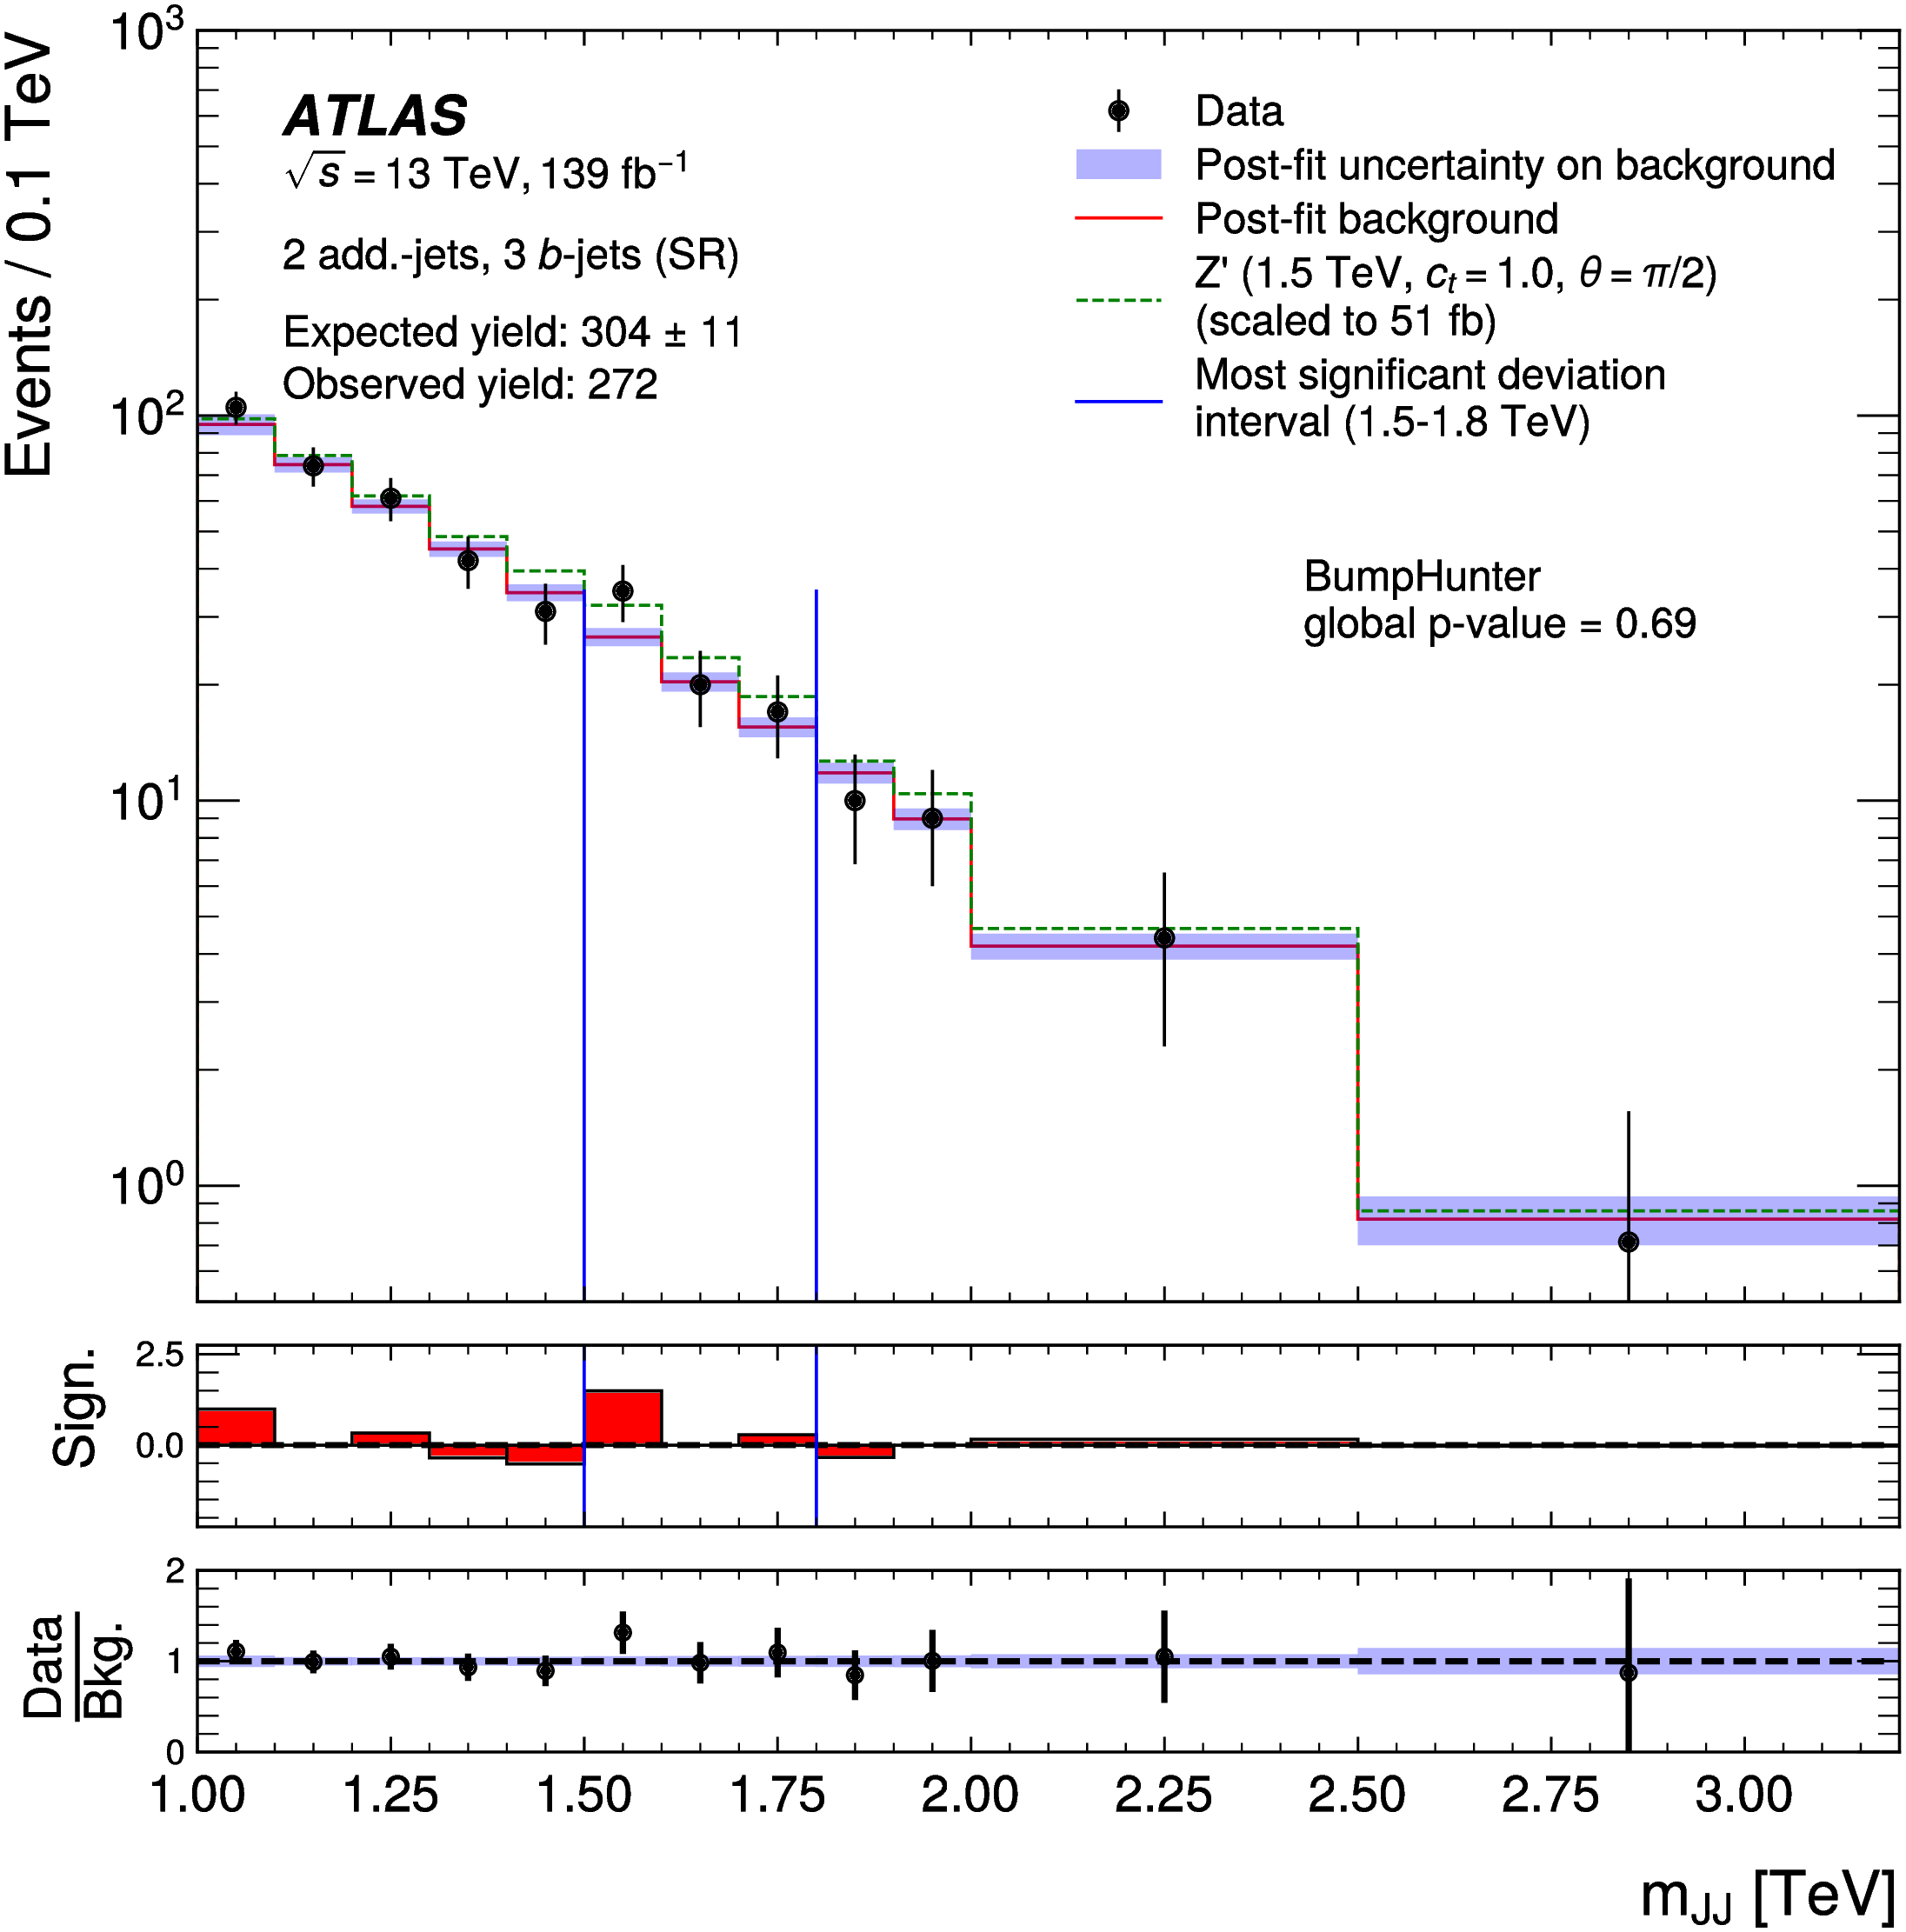
\includegraphics[width=\textwidth]{bump}
         \caption{}
         \label{fig:bump}
     \end{subfigure}
     \begin{subfigure}[b]{0.32\textwidth}
         \centering
         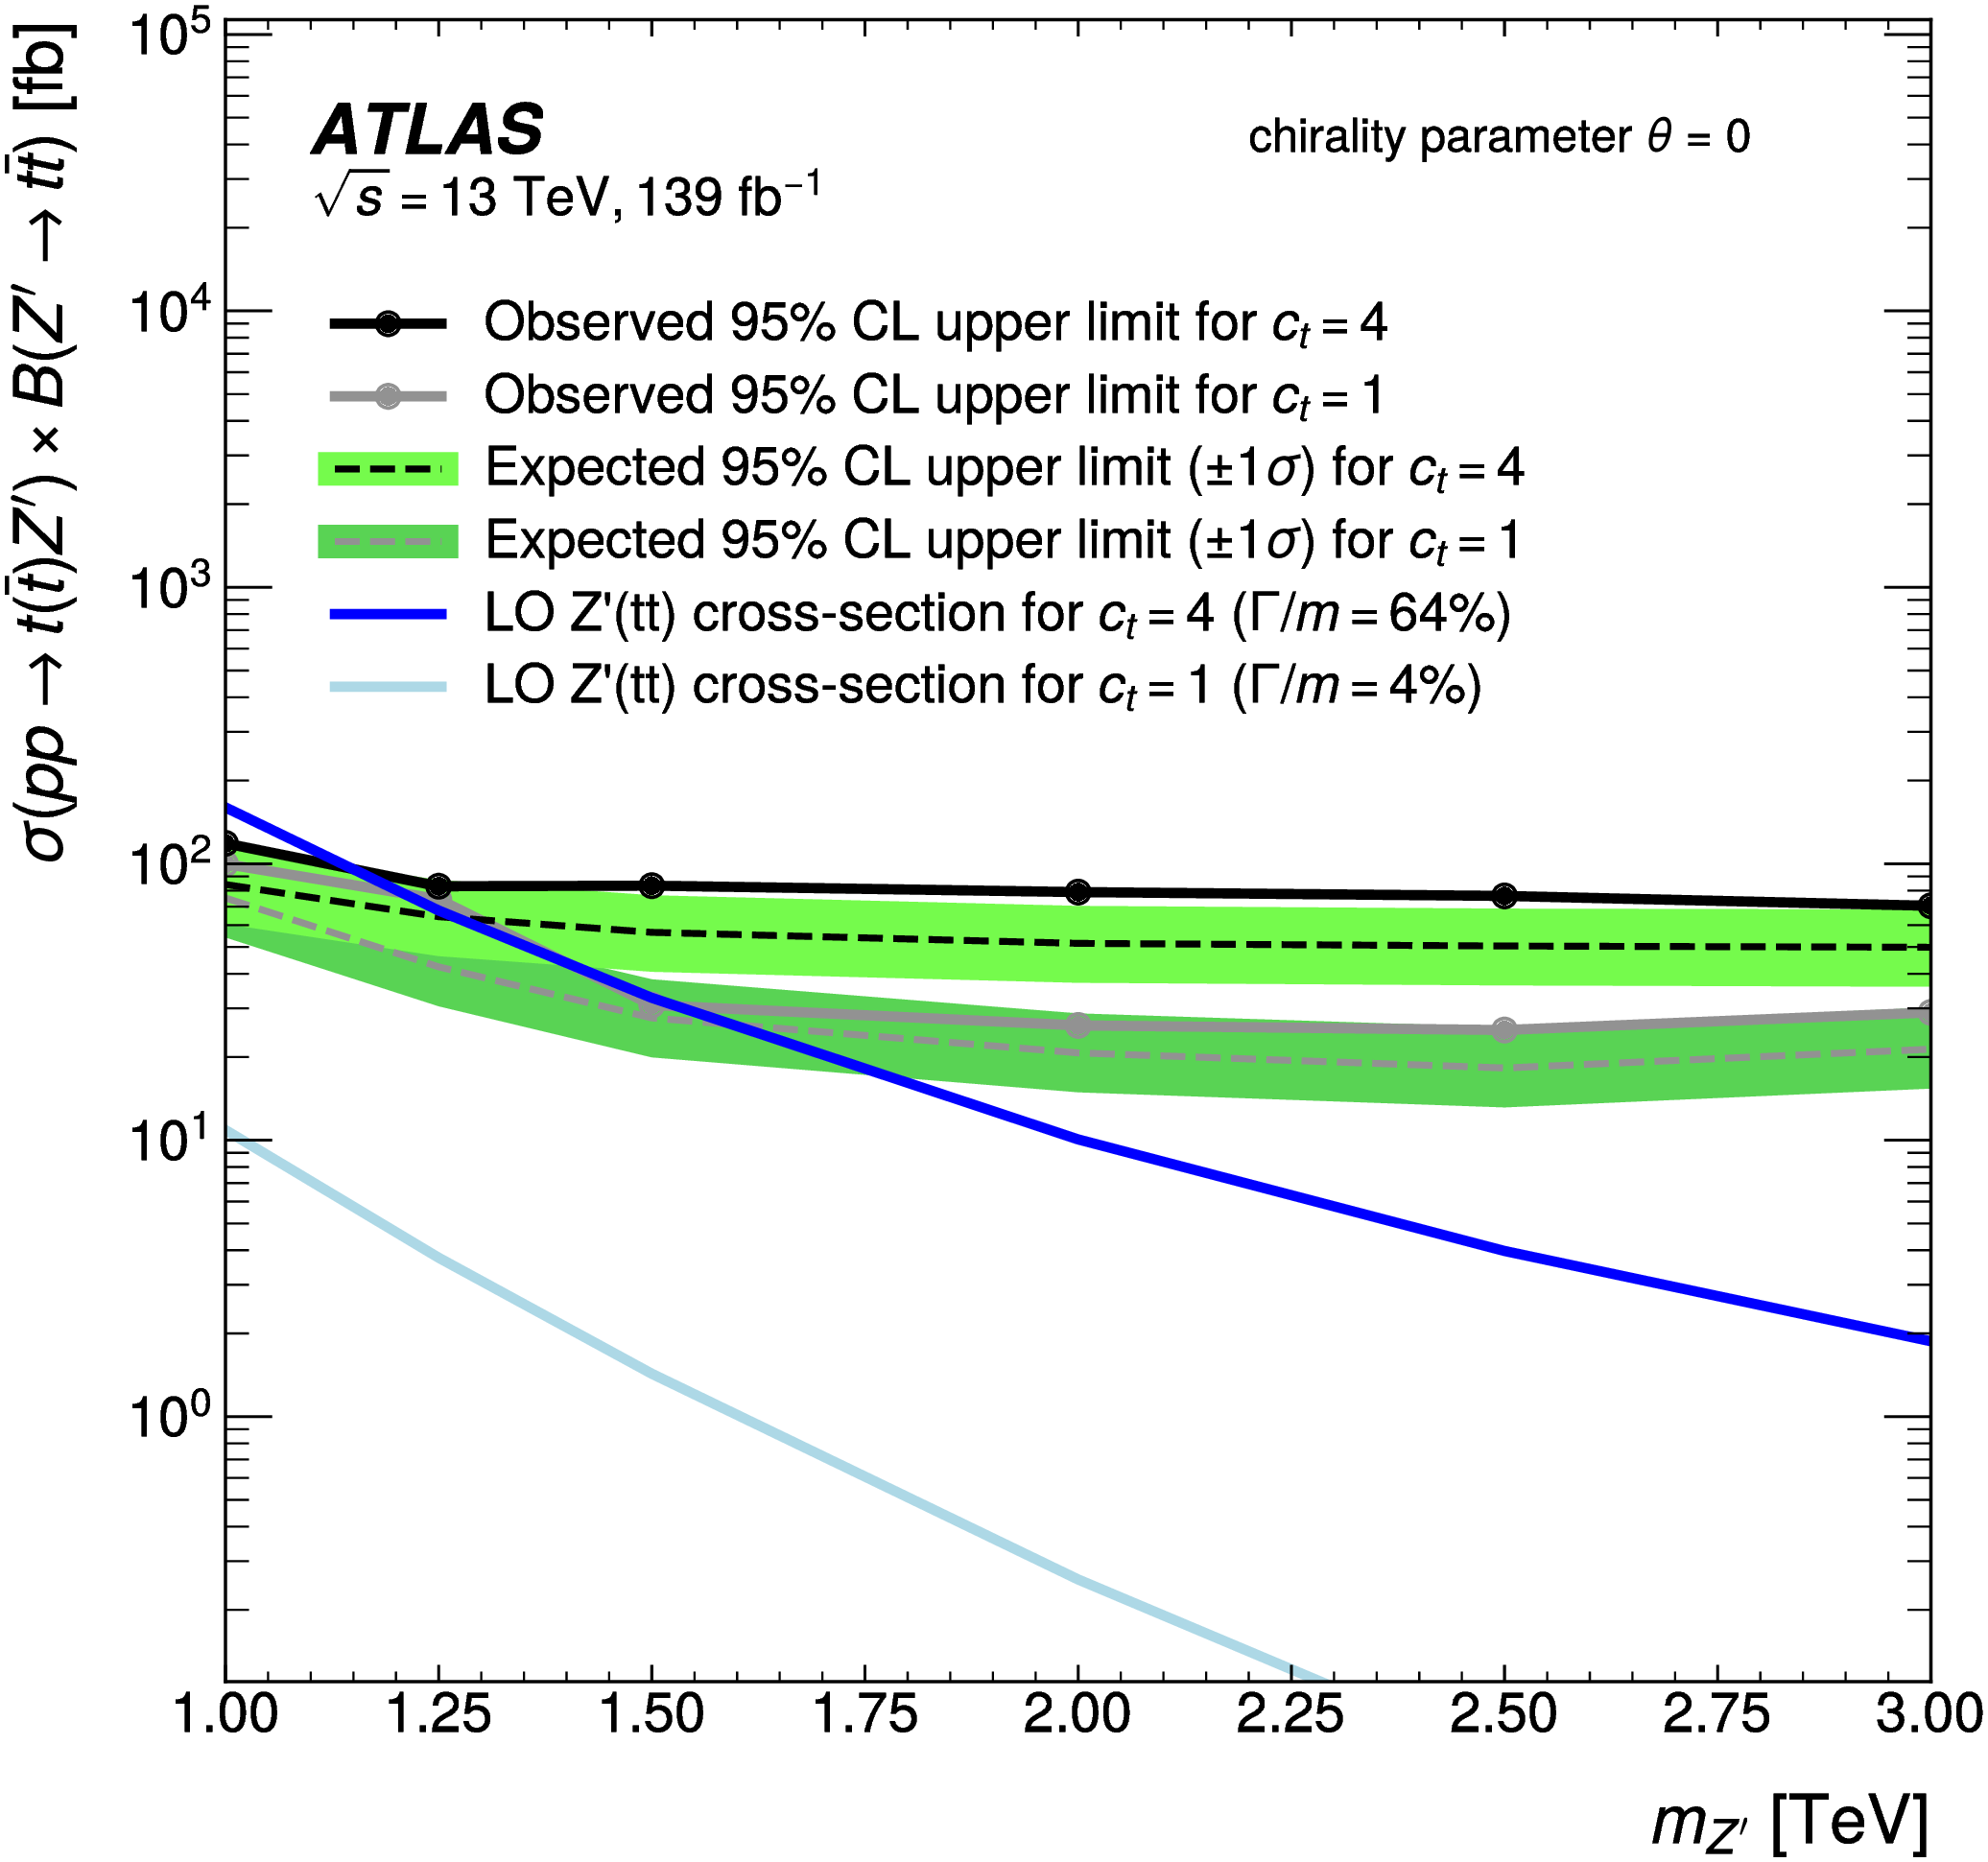
\includegraphics[width=\textwidth]{tttt}
         \caption{}
         \label{fig:ttttlimits}
     \end{subfigure}
        \caption{tttt}
        \label{fig:tttt}
\end{figure}



\begin{figure}[htp]
     \centering
     \begin{subfigure}[b]{0.32\textwidth}
         \centering
         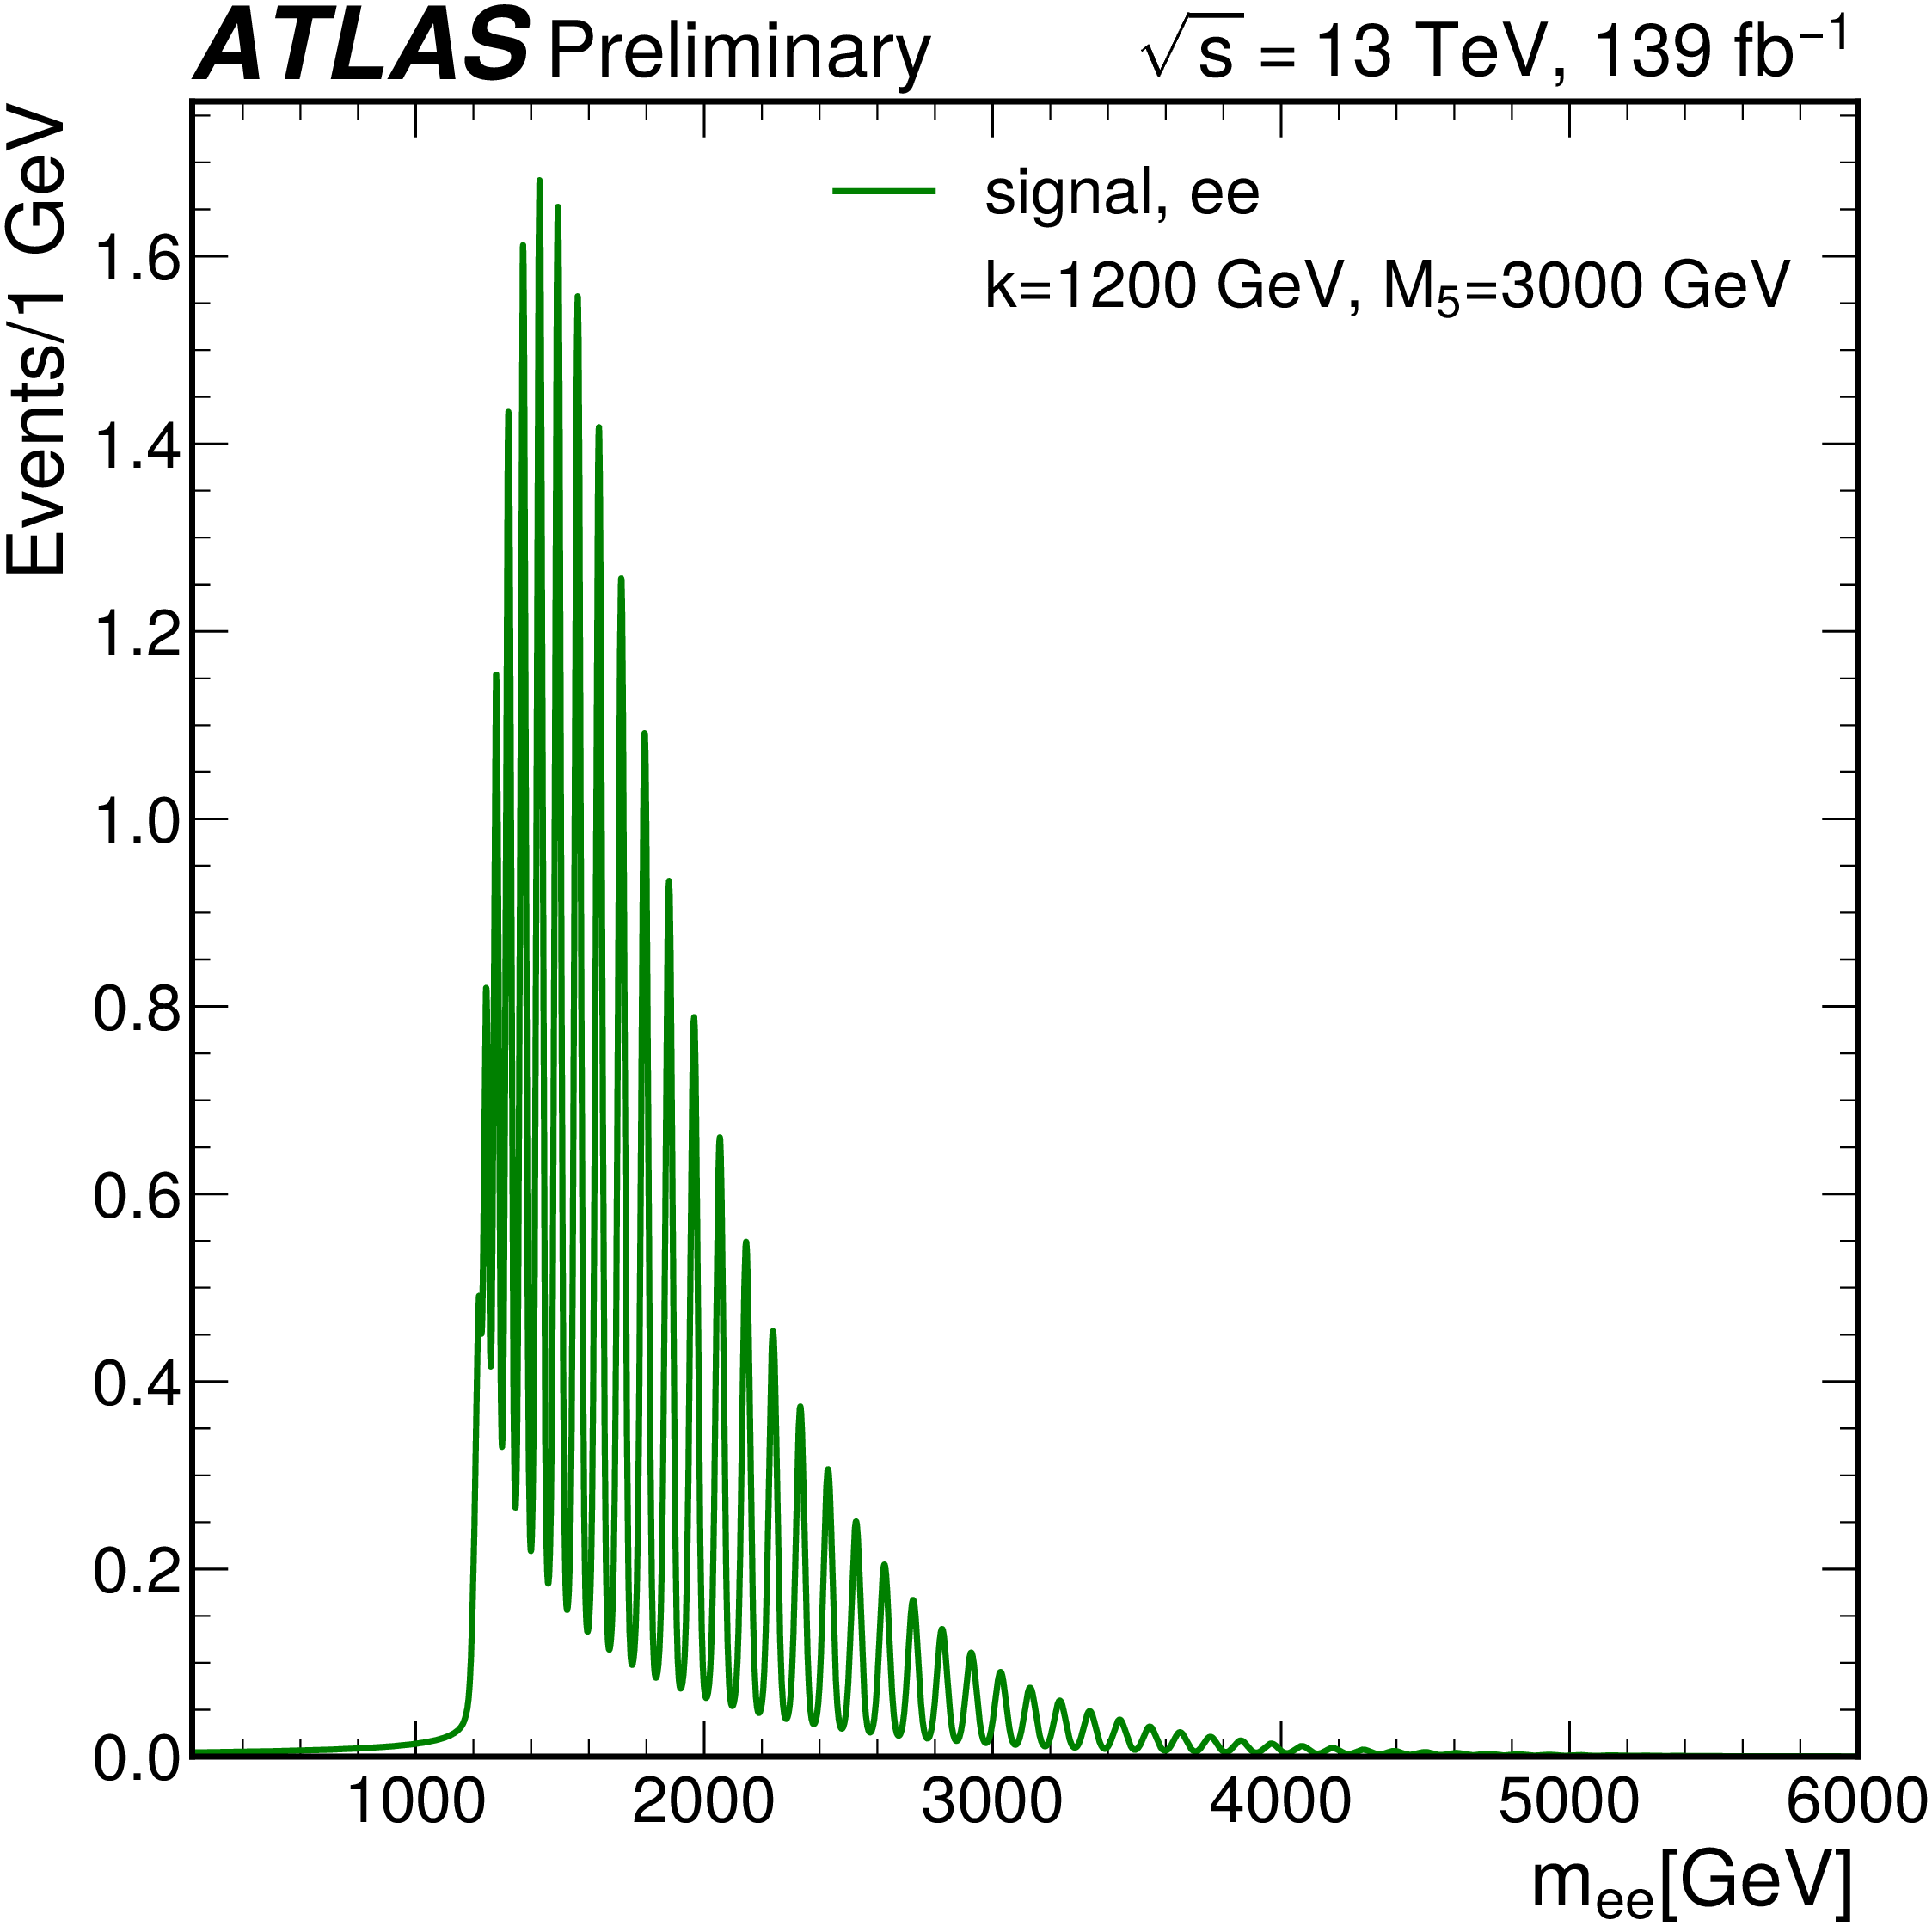
\includegraphics[width=\textwidth]{signal}
         \caption{}
         \label{fig:signal}
     \end{subfigure}
     \begin{subfigure}[b]{0.32\textwidth}
         \centering
         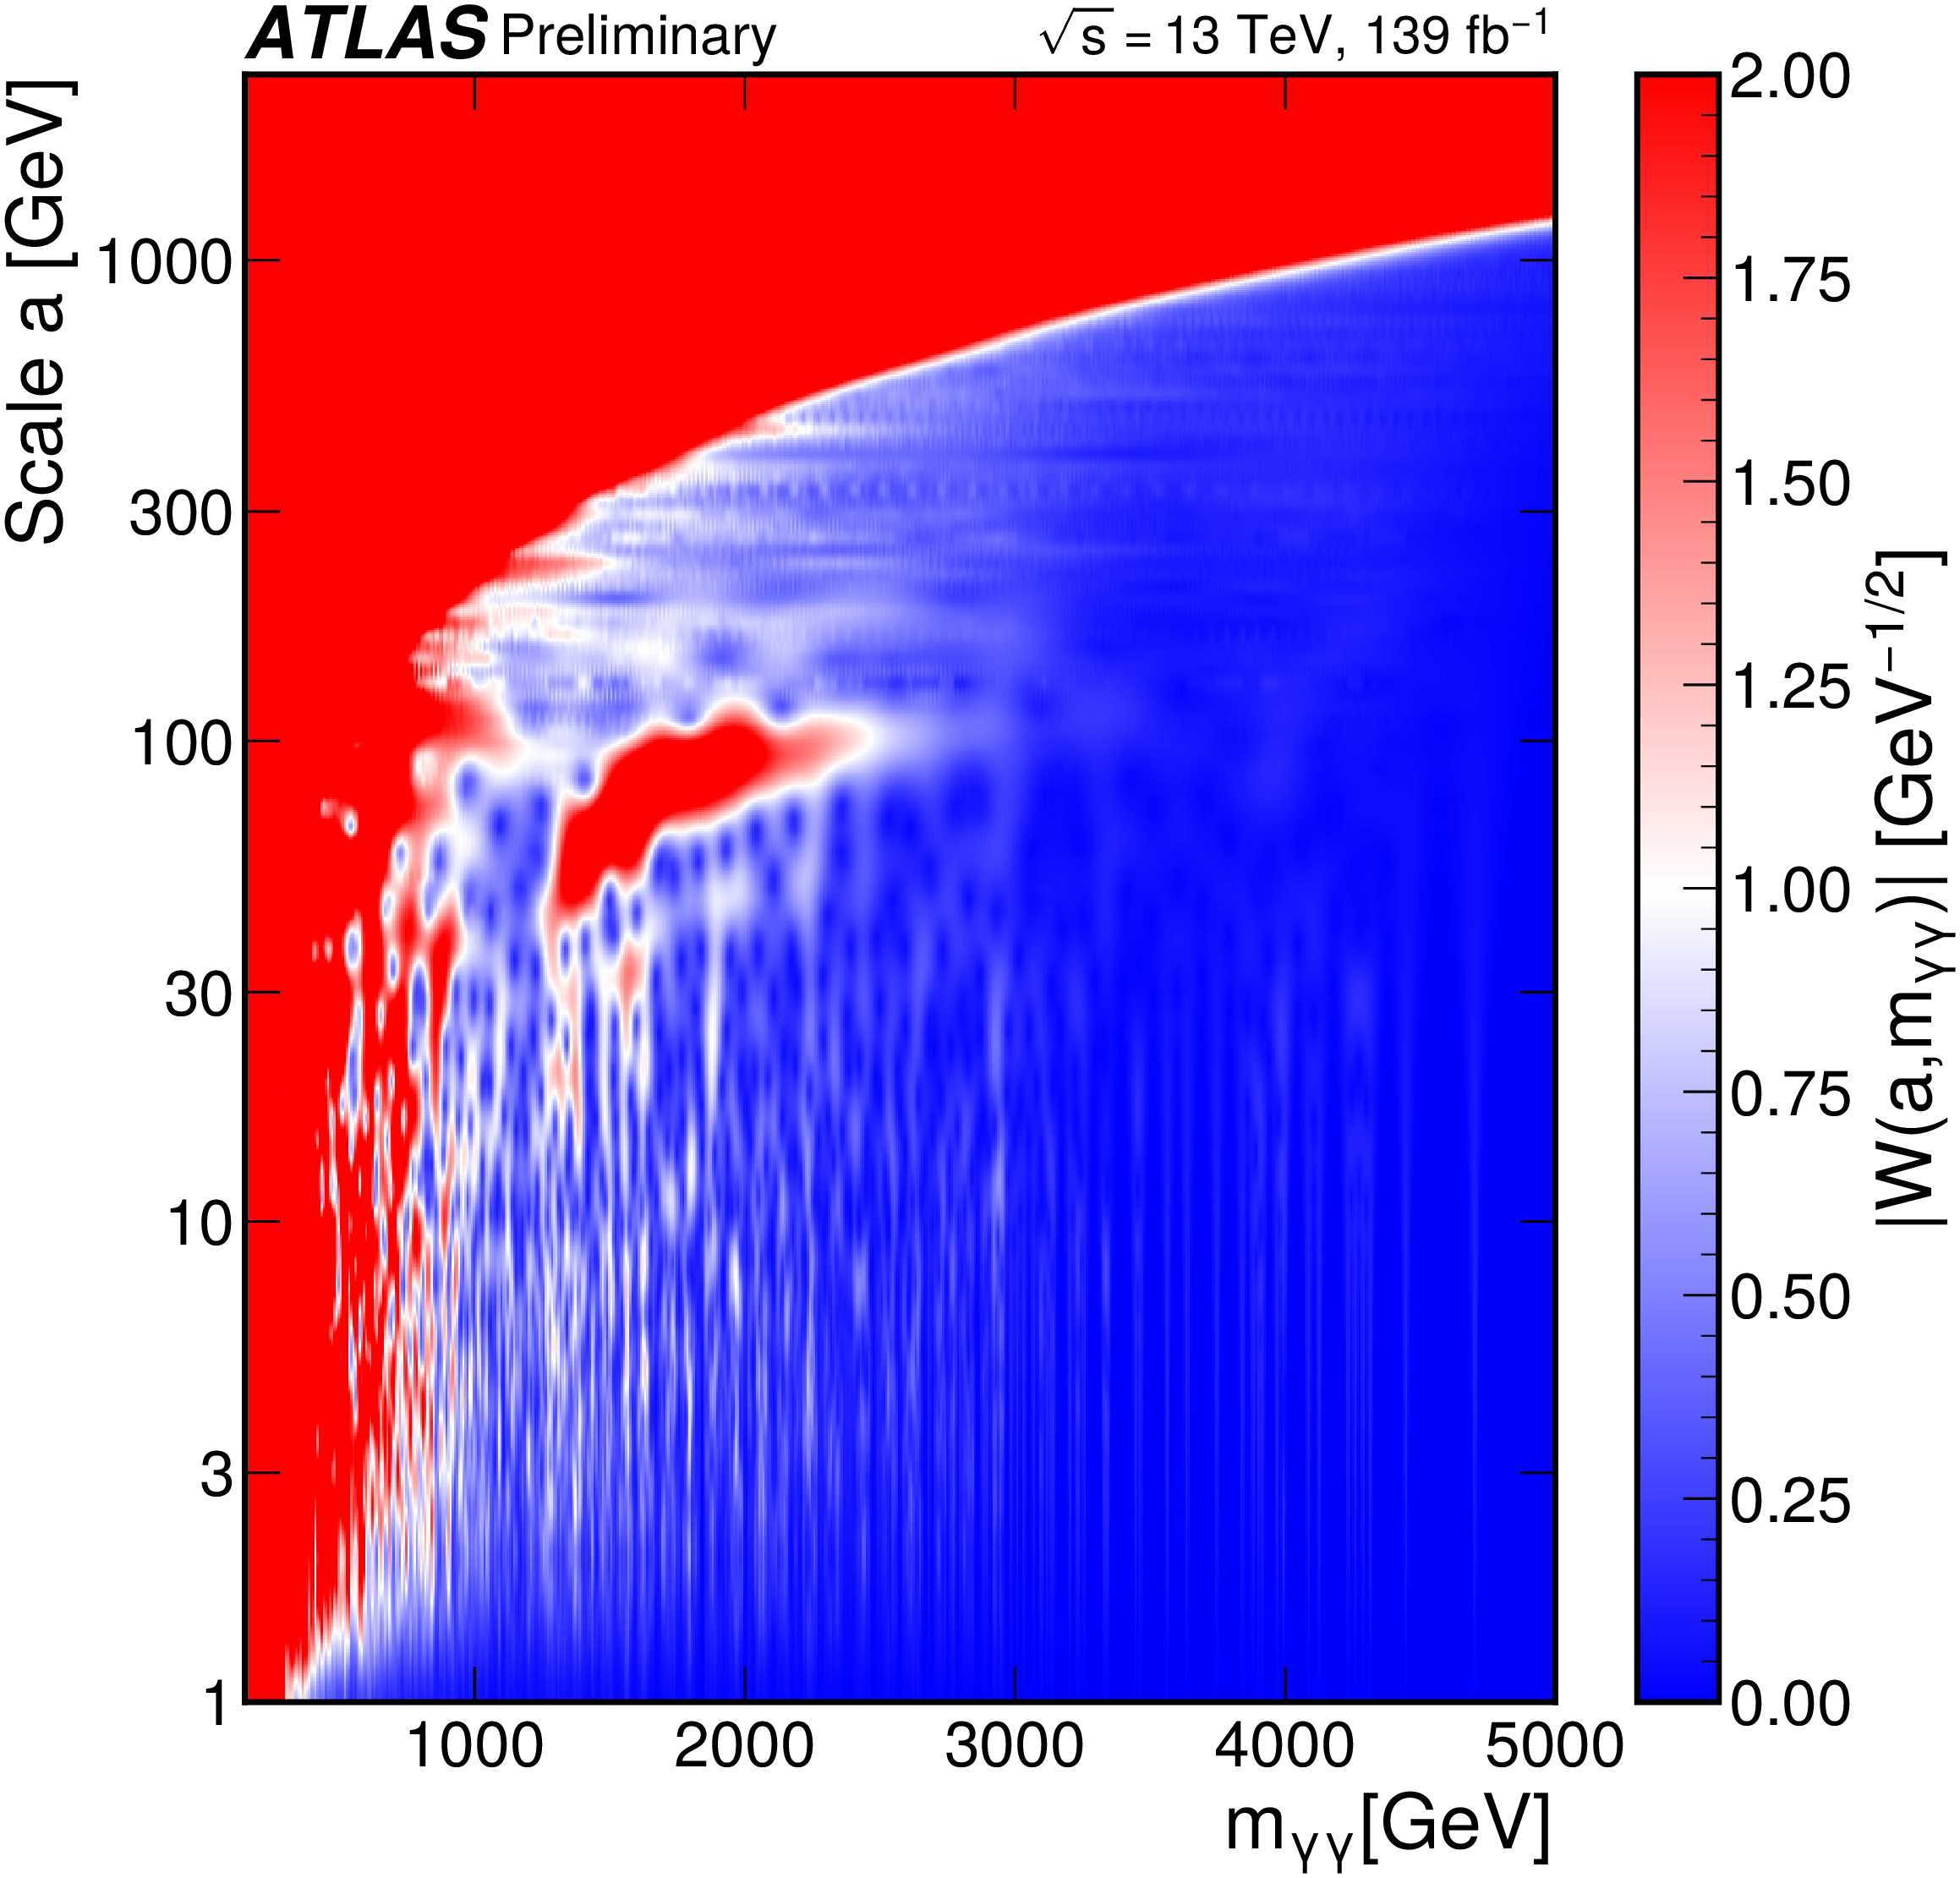
\includegraphics[width=\textwidth]{bkgsig}
         \caption{}
         \label{fig:shape}
     \end{subfigure}
     \begin{subfigure}[b]{0.32\textwidth}
         \centering
         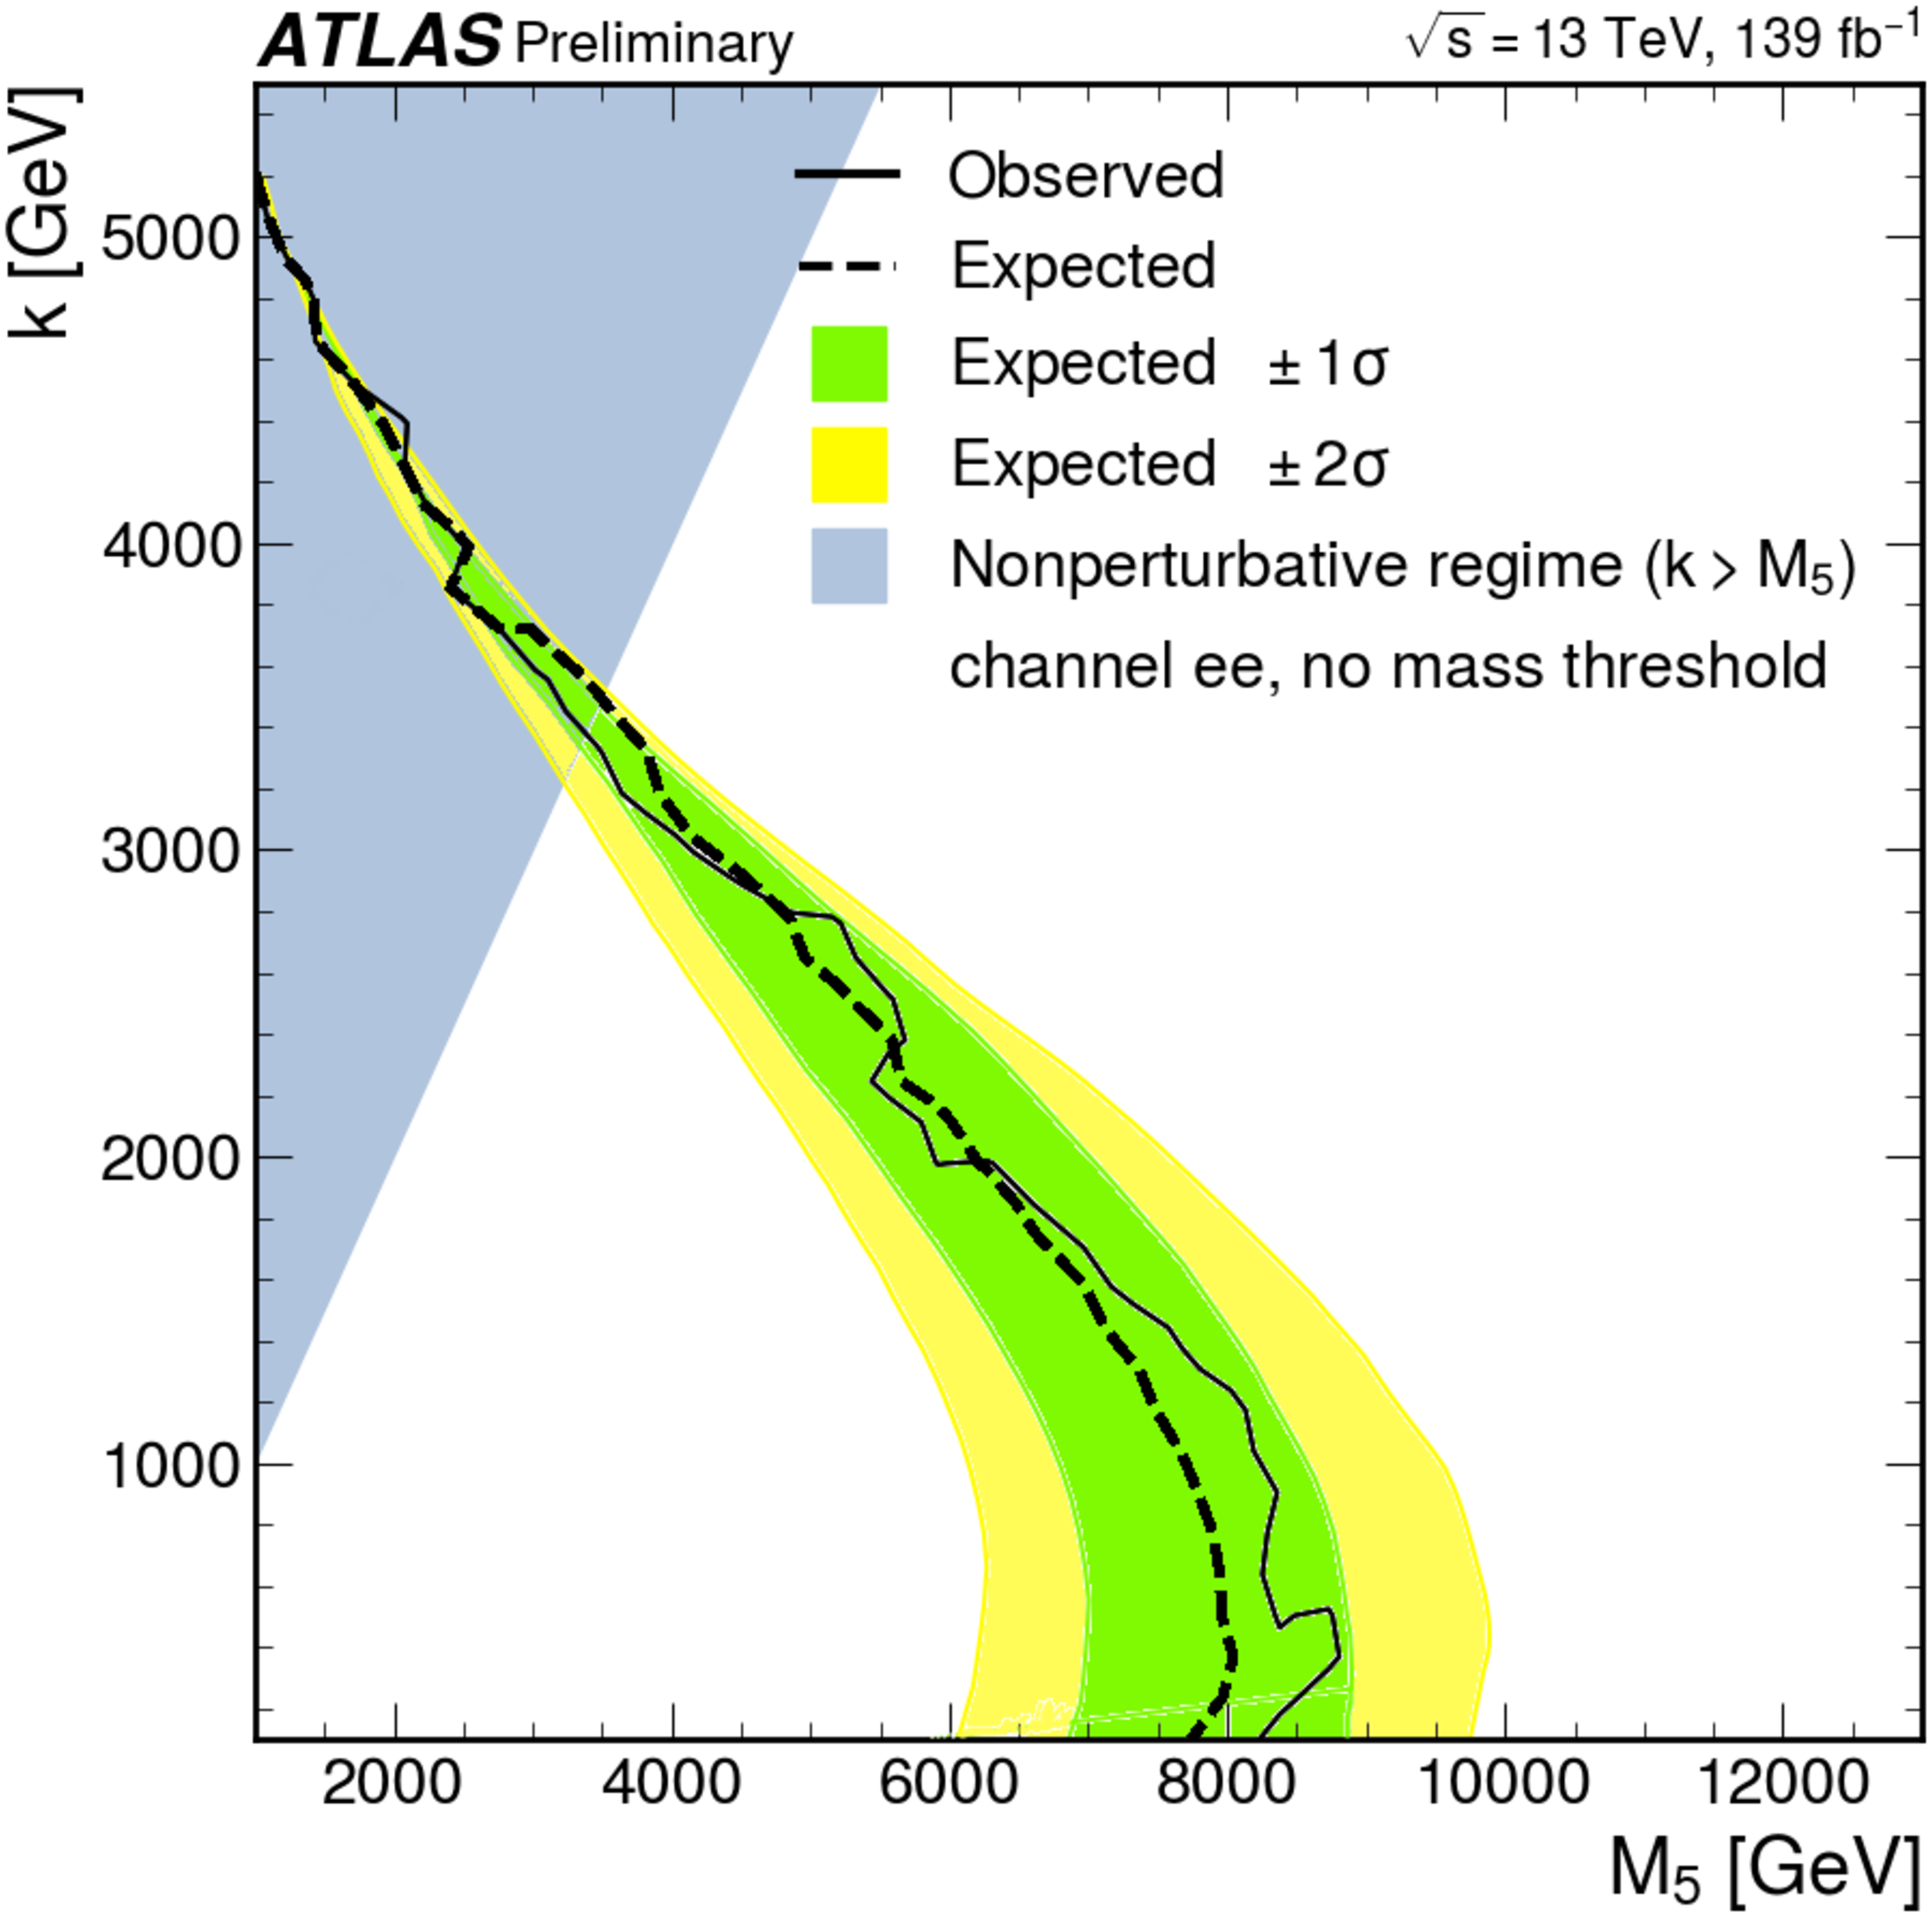
\includegraphics[width=\textwidth]{periodic}
         \caption{}
         \label{fig:perlimits}
     \end{subfigure}
        \caption{Periodic}
        \label{fig:periodic}
\end{figure}




\section*{References}

\begin{thebibliography}{99}
\bibitem{ja}C Jarlskog in {\em CP Violation}, ed. C Jarlskog
(World Scientific, Singapore, 1988).

\bibitem{ma}L. Maiani, \Journal{\PLB}{62}{183}{1976}.

\bibitem{bu}J.D. Bjorken and I. Dunietz, \Journal{\PRD}{36}{2109}{1987}.

\bibitem{bd}C.D. Buchanan {\it et al}, \Journal{\PRD}{45}{4088}{1992}.

\end{thebibliography}

\end{document}

%%%%%%%%%%%%%%%%%%%%%%
% End of moriond.tex  %
%%%%%%%%%%%%%%%%%%%%%%


%%% Local Variables: 
%%% mode: latex
%%% TeX-master: t
%%% End: 

%%% Local Variables: 
%%% mode: latex
%%% TeX-master: t
%%% End: 

%%% Local Variables: 
%%% mode: latex
%%% TeX-master: t
%%% End: 
